\documentclass[fleqn,usenatbib]{mnras}
%
% Version of 18-07-15, based on version 25-April-2014 of Bamberg abstract template
%
% do not exceed one page in the compiled version
% do not change the page format, font size, etc.
%
%\pdfoutput=1
%\bibliographystyle{mnras}
\usepackage{newtxtext,newtxmath}
\usepackage[T1]{fontenc}
\usepackage{csvsimple}
\DeclareRobustCommand{\VAN}[3]{#2}
\let\VANthebibliography\thebibliography
\def\thebibliography{\DeclareRobustCommand{\VAN}[3]{##3}\VANthebibliography}

\usepackage{twoopt}
%\usepackage[colorlinks,linkcolor=blue,urlcolor=blue,citecolor=black]{hyperref} %% to avoid \citeads line fills
%\bibpunct{(}{)}{;}{a}{}{,}             %% natbib format for A&A and ApJ
%\makeatletter
%  \newcommandtwoopt{\citeads}[3][][]{\href{http://ui.adsabs.harvard.edu/abs/#3}%
%    {\def\hyper@linkstart##1##2{}%
%     \let\hyper@linkend\@empty\citealp[#1][#2]{#3}}}
  %\newcommandtwoopt{\citepads}[3][][]{\href{http://ui.adsabs.harvard.edu/abs/#3}%
  %  {\def\hyper@linkstart##1##2{}%
  %   \let\hyper@linkend\@empty\citep[#1][#2]{#3}}}
  %\newcommandtwoopt{\citetads}[3][][]{\href{http://ui.adsabs.harvard.edu/abs/#3}%
  %  {\def\hyper@linkstart##1##2{}%
  %   \let\hyper@linkend\@empty\citet[#1][#2]{#3}}}
%   \newcommandtwoopt{\citeauthorads}[3][][]%
%    {\href{http://ui.adsabs.harvard.edu/abs/#3}
%    {\def\hyper@linkstart##1##2{}%
%     \let\hyper@linkend\@empty\citeauthor[#1][#2]{#3}}}
%  \newcommandtwoopt{\citeyearads}[3][][]%
%    {\href{http://ui.adsabs.harvard.edu/abs/#3}
%    {\def\hyper@linkstart##1##2{}%
%     \let\hyper@linkend\@empty\citeyear[#1][#2]{#3}}}
%  \renewcommand*\aa@pageof{, page \thepage{} of \pageref*{LastPage}} % to get rid of "Package hyperref Warning: Suppressing link with empty target on input line 92." warnings
%\makeatother
%\usepackage[varg]{txfonts}
% \usepackage{grffile} % Allowing includegraphics to include files with arbitrary filenames
\usepackage{pdflscape} % Produce landscape pages in a (mainly) portrait document -> Useful, for example, with large multipage tables, and is compatible with the packages longtable
%
\usepackage{booktabs}
\usepackage{csvsimple}
\usepackage{pgfplotstable}
\usepackage{array}
%\usepackage{colortbl}
\usepackage{amsmath}
\usepackage{amsfonts}
\usepackage{dsfont}
\usepackage{amsxtra}
\usepackage{hyperref}
\usepackage{amssymb}
\usepackage{upgreek}
\usepackage{comment}

\usepackage{multirow}
\usepackage{url}

\usepackage{graphicx,epsfig}
%\usepackage{dcolumn}
%\usepackage{bm}
%\usepackage{ulem}

\usepackage{xspace} 
%\usepackage[textwidth=16cm]{geometry}
%\geometry{a4paper}

\pagestyle{empty}
%
\textwidth 17.0cm
\textheight 23.0cm
%\oddsidemargin -1.0cm
\topmargin -1.0cm
%\usepackage{natbib,twoopt}
\usepackage{lscape}
%\bibpunct{(}{)}{;}{a}{}{,}             %% natbib format ftor A&A and ApJ
%\newcommand{\bain}{Bulletin of the Astronomical Institutes of the Netherlands}
%\newcommand{\nat}{Nature}
%\newcommand{\aap}{Astron. Astrophys.}
%\newcommand*\aaps{A\&AS}
%\newcommand{\pasa}{PASA}
%\newcommand{\aua}{Astron. Astrophys.}
%\newcommand{\aasup}{\it Astron.\ Astrophys.\ Suppl.}
%\newcommand{\apjl}{Astrophys.\ J.\ Letters}
%\newcommand{\apj}{Astrophys.\ J.}
%\newcommand{\aj}{Astron.\ J.}
%\newcommand{\apjs}{Astrophys.\ J.\ Suppl.}
%\newcommand{\araa}{Ann.\ Rev.\ Astron.\ Astrophys.}
%\newcommand{\rmxaa}{RMxAA}
%\newcommand{\jqsrt}{\it J. Quant. Spectrosc. Rad. Transfer}
%\newcommand{\mnras}{Monthly Notices Roy. Astron. Soc.} 
%\newcommand{\rmph}{Rev. Mod. Phys.}
%\newcommand{\pasp}{{Publ. Astron. Soc. Pacific} }
%\newcommand{\nar}{{New Astronomy Review}}
\usepackage{subfig}
\usepackage{xcolor}
\usepackage{lineno}
\linenumbers
% 
%	\usepackage[
%	backend=bibtex,
%	style=alphabetic,
%	citestyle=alphabetic
%	]{biblatex}
%\addbibresource{references.bib}

% 

%
%%% Talk / Poster (uncomment relevant line)
%
%{\small Talk} \\[3mm]   %% Contributed talk
%{\small Poster} \\[3mm]             %% Poster 
%
\title[Mass Model Updates]{Mass Model Updates}

% The list of authors, and the short list which is used in the headers.
% If you need two or more lines of authors, add an extra line using \newauthor
\author[Aakash Bhat]{
Aakash Bhat$^{1}$\thanks{E-mail: aabhat@astro.physik.uni-potsdam.de}
\\
% List of institutions
$^{1}$Institute of Physics and Astronomy, University of Potsdam, Karl-Liebknecht-Str. 24/25, 14476, Potsdam, Germany
}

% These dates will be filled out by the publisher
\date{Accepted XXX. Received YYY; in original form ZZZ}

% Enter the current year, for the copyright statements etc.
\pubyear{2023}

 
\begin{document}
\label{firstpage}
\pagerange{\pageref{firstpage}--\pageref{lastpage}}
\maketitle
\begin{abstract}


s

\end{abstract}


\begin{keywords}
galactic dynamics --
milky way --
\end{keywords}


   
   
%\tableofcontents
%\newpage
\section{Introduction}

Mass models include \citet{2017MNRAS.465...76M},\citet{2017OAst...26...72B}, \citet{1998MNRAS.294..429D}
\section{Observational constraints}
\subsection{Solar circle}

Distance of Sun from the Galactic center from \citet{2019A&A...625L..10G} :

\begin{equation}
    r_\odot=8.178\pm 0.035 \mathrm{kpc}
\end{equation}

\subsection{Velocity Curve}

The velocity curve of the Milky way is amongst the most powerful observational constraints for any model of the Galaxy. Since the last update, many new measurements have been published mainly due to the precision obtained due to the \textit{Gaia} mission, especially the second data release \citet{2018A&A...616A...2L}. The circular velocity curve for a potential $\phi$ in a cylindrical coordinate system can be calculated using the radial force, which is given as
\begin{equation}
v^2_{\mathrm{circ}} = r\times|{-\frac{\partial\phi}{\partial r}}|_{z=0}
\end{equation}

The observational data is gathered differently depending upon the distance from the centre. Inside 5 kpc from the centre studies are based on HI or CO line emissions which use the tangent velocity methods. The middle range of 5-25 kpc relies on values of star forming regions, cepheids, etc. On the other hand outside the limit of the solar circle halo tracers are used. 

In this work we chose 5 different studies. For distances below 5 Kpc we used the data provided by three different studies. These are:
\begin{enumerate}
    
    \item The rotation velocities from \citet{2009PASJ...61..227S} which relied on CO and HI values from \citet{1978A&A....63....7B} and \citet{1985ApJ...295..422C}. We don't take values which lack uncertainties. This is referred to as RC1 from here.
    \item The second study is from \citet{2021PASJ...73L..19S}. This updated rotation curve is different from the previous one lacking the characteristic bulge feature within the inner Milky Way. This is RC2.
    \item The last studies are from \citet{2014ApJ...783..130R} and \citet{2019ApJ...885..131R}. We used parameters provided in Tab. \ref{tab:params} to calculate the Galacto-centric positions and velocities of these star forming regions using the galpy package in python \citet{2015ApJS..216...29B}. Errors are estimated by sampling the parameters a million times using the uncertainties on the parameters of the SFRs as well as the Galactic parameters. For the latter, systematic uncertainties are also taken into account, as in the case of the circular velocity of the sun from \citetads{2019ApJ...871..120E} where $5\%$ uncertainties were added. Similarly we add systematic uncertainties to the LSR values taken from \citet{2013ApJ...779..115B}. This is referred to as RC3.
\end{enumerate}


For distances between 5-25 Kpc we rely on the rotation curve from \citet{2019ApJ...871..120E}. Since this is the most well studied region and the rotation curve is most precise here, we stick to the values used in their study for any priors on the distance of the sun and the circular velocity in our paper. 

For distances of 25-200 kpc we get data from \citet{2014ApJ...785...63B}. While the data was calculated for three different values of radius and velocity of the sun, we chose the middle value. As shown by \citet{2014ApJ...785...63B}, the rotation curve is not as sensitive to the radius and circular velocity of the sun in this region, and any changes are well within the uncertainties. Furthermore, while equation 2 of \citet{2014ApJ...785...63B} does not hold for larger values of R, as the conversion leads to negative values of the rotation velocity, we use it for the inner rotation curve for new (R$_o$,V$_o$) values.
\begin{table}
    \centering
    \begin{tabular}{|c|c|}
        \hline
        Parameter&Values\\
        \hline
        \hline
        $r_\odot$ & $8.178\pm 0.035$ \\
        $v_\odot$ & $229 \pm 0.2$ \\
        U & $11.1 \pm 1.69$ \\
        V & $12.24 \pm 2.47$ \\
        W & $7.25 \pm 0.87$ \\
        \hline
    \end{tabular}
    \caption{Parameters used to estimate circular velocities for the SFRs of \citet{2019ApJ...885..131R} as well as the shift for the inner 5 kpc.}
    \label{tab:params}
\end{table}

\begin{equation}
    V_\text{new}(R)=V_\text{old}\times\frac{R_{\text{old}}}{R_{\text{new}}} + (\omega_\text{new}-\omega_\text{old})\frac{R}{R_\text{new}}
\end{equation}



\subsection{Vertical Force}

The vertical force is another important observation which allows to constrain the potential in the perpendicular direction. Just like the circular velocity which is given by the radial acceleration, the vertical force is defined as
\begin{equation}
        K_{z}=-\frac{\partial\phi}{\partial z}
\end{equation}

We used the measurements of the vertical force from \citet{2013ApJ...779..115B}, taken at $z = 1.1 $kpc.

\subsection{Matter density at the solar circle}
Despite the fact that we have both forces, the constraint of matter density is important to properly constrain the values. When using only the forces, the uncertainties on the individual parameters were found to be much higher, and the disk scale height $b_d$ was found to be $>1$ kpc at the best fit. This is due to the fact that when dealing with forces, there is a big correlation between the masses and the scale length(or heights) of the various models. To resolve this we add one extra measurement in the residual, which is the local matter density. The local matter density leads to a convergence in the phase space of masses and scale heights. We therefore use the value of $\rho_\odot = 0.097 \pm 0.013$ and dark matter density of $\rho_\odot = 0.013 \pm 0.003$ from \citet{2015ApJ...814...13M}. This matches the value of 0.011 from \citet{2010A&A...523A..83S} and 0.014 from \citet{2014A&A...571A..92B}), where the increase comes from an increase of solar radius considered, as the dark matter density increases outward of the solar circle. Without the use of this value for fitting, our best fits lead to a value which was almost half of this value.
\section{Fitting Procedure}

We use the Lmfit module \citep{newville_matthew_2014_11813} to fit the curves. The residual function uses the chi-square where we weigh the data by the number of measurements, such that the residuals are multiplied by a factor of $1/\sqrt{N}$, where $N$ is the number of measurements from one study. We therefore have,
\begin{equation}
    \text{Residual}= \frac{1}{\sqrt{N_j}}\frac{(Data-Model)}{\sigma}
\end{equation}
The sum of squares is then used to calculate the weighted chi-square by the lmfit module.
We use the Ampgo solver to get the best-fit. The initial values for the fit are taken from \citet{andreassmass}. Since the parameters are highly correlated the uncertainties are then estimated using an MCMC procedure which evaluates the function $10^6$ times (100 walkers with 10000 steps each) using the final values of the apmgo solver as the initial point. Due to the high correlations, we report the uncertainties along with the mode of the MCMC posterior distributions. To avoid sampling in non-physical regions, we provide maximum values for scale heights of the bulge, disk, and halo components, and burn 1000 samples, which is roughly twice the auto-correlation time. We also check for the median acceptance rate to be above 0.2. The mode of the MCMC distribution is reported along with the high and low density intervals, which are calculated after fitting the posterior distributions individually.
\section{Results}

\subsection{Model I: Allen Santillan}

Model I has Bulge and disk from Miyamoto and Nagai and dark matter halo is taken from Allan and Santillan and modified to the form in \citet{andreassmass}.

 In our fitting procedure, we start with $\Lambda$ = 100 kpc instead of 200, since we do not have any data points outside of 200 kpc. The maximum value is however not allowed to vary more than 200 kpc, like was done in the previous model. Due to the high level of correlation, the median of the MCMC procedure is different from the maximum likelihood estimate. The update of this model with RC1 is closest to the previous model employed by \citet{andreassmass} due to the similarity of the curve used for the estimation of inner 5 kpc of the Milky Way, showing the characteristic bulge feature missing in RC2 and RC3. This change leads to a significant shift in the scale length of the bulge in RC2 and RC3 as reported in \ref{tab:model1params}, leading to an average of 3.49 kpc for RC2 and RC3, as opposed to 0.224 kpc for RC1. This also leads to an increase in the mass within the scale height of the bulge.
 
 For the disc, the masses are within the error limits of the three curves. However, RC3 gives a much bigger scale length, while all three rotation curves leads to a much bigger scale height for the disk. The errors on the latter are also quite large and a smaller disk is not excluded.
 
 For the halo, the masses are predicted to be close to the initial value and similar for all three. However, all three curves predict a much bigger scale length $a_h$, close to the maximum allowed value of 20 kpc. Similarly, a much smaller $\Lambda$ is preferred, which however cannot directly be compared with \citetads{andreassmass} where it was not allowed to vary. The fits to the rotation curves and the vertical forces are given in \ref{fig:Model1_rc} and \ref{fig:Model1_vertif}


 \pgfplotstableread[col sep=comma]{Model_I/output_params/fit_all_10000_100_params.csv}\tableaf
\begin{table*}
\centering
\caption{Fitted parameters values for Model I.}
\label{tab:model1params} 
\renewcommand{\arraystretch}{1.1}
\resizebox{0.9\textwidth}{!}{
\pgfplotstabletypeset[
columns={Parameter,ampgo_1,mcmc_mxl_1,mcmc_mode_1,ampgo_2,mcmc_mxl_2,mcmc_mode_2,ampgo_3,mcmc_mxl_3,mcmc_mode_3},
column type=c,
string type,
every head row/.style={before row={\hline\hline&\multicolumn{3}{c}{RC1}&\multicolumn{3}{c}{RC2}&\multicolumn{3}{c}{RC3}\\},after row=\hline,},
every last row/.append style={after row={\hline} },
every first column/.style={column type/.add={}{}},
every last column/.style={column type/.add={}{}},
columns/Parameter/.style={column name=Name,string replace*={_}{\textunderscore}},
columns/ampgo_1/.style={column name=Ampgo,column type=c,numeric type,fixed,precision=2},
columns/mcmc_mxl_1/.style={column name=MCMC MXL,column type=c,numeric type,fixed,precision=2},
columns/mcmc_mode_1/.style={column name=MCMC Mode,column type=c,numeric type,fixed,precision=2},
columns/ampgo_2/.style={column name=Ampgo,column type=c,numeric type,fixed,precision=2},
columns/mcmc_mxl_2/.style={column name=MCMC MXL,column type=c,numeric type,fixed,precision=2},
columns/mcmc_mode_2/.style={column name=MCMC Mode,column type=c,numeric type,fixed,precision=2},
columns/ampgo_3/.style={column name=Ampgo,column type=c,numeric type,fixed,precision=2},
columns/mcmc_mxl_3/.style={column name=MCMC MXL,column type=c,numeric type,fixed,precision=2},
columns/mcmc_mode_3/.style={column name=MCMC Mode,column type=c,numeric type,fixed,precision=2},
]{\tableaf}
}
\tablefoot{I}
\end{table*}


\begin{figure}
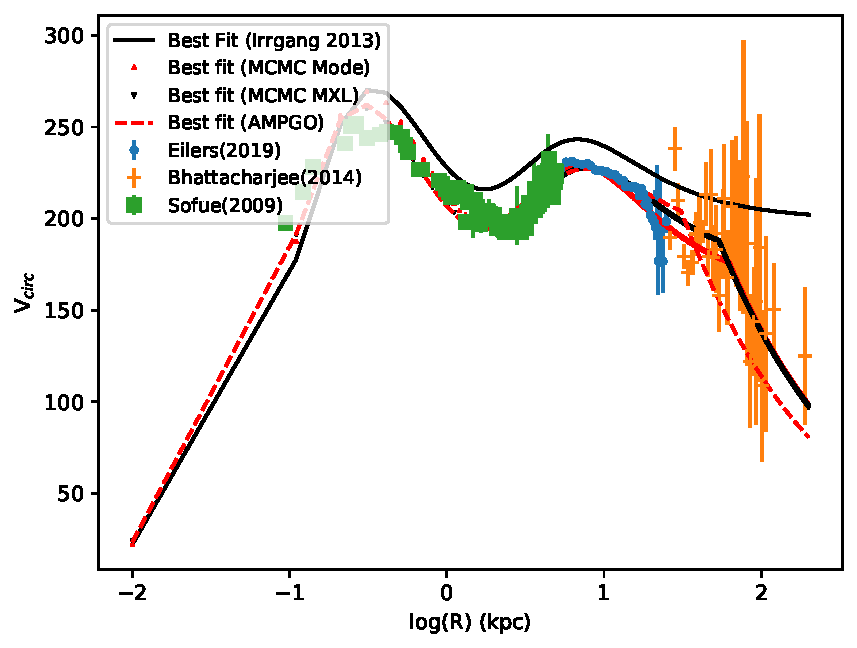
\includegraphics[width=\columnwidth]{Model_I/Plots/Sofue(2009)/Rotcur_ModelI_eil_bhatta_log_10000_100.pdf}
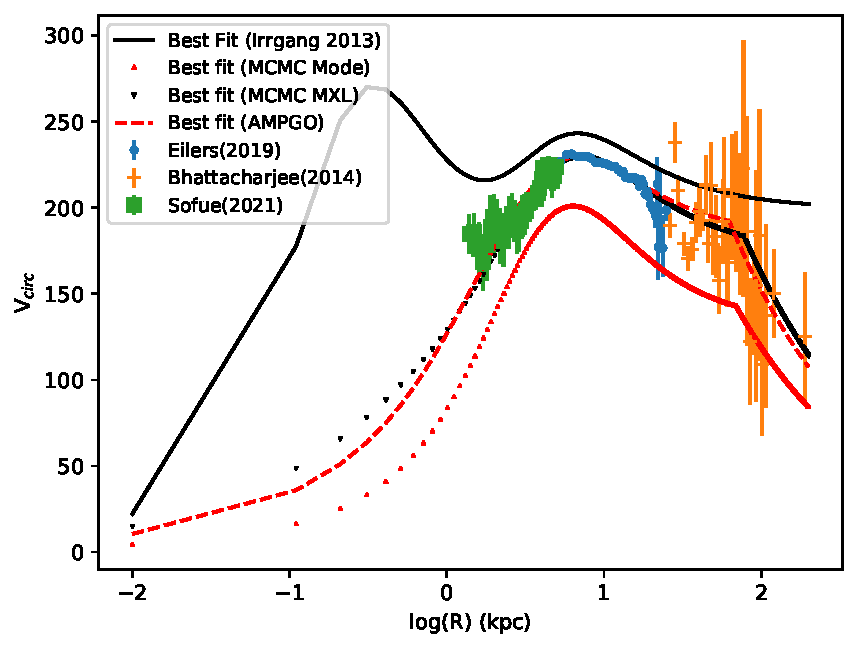
\includegraphics[width=\columnwidth]{Model_I/Plots/Sofue(2021)/Rotcur_ModelI_eil_bhatta_log_10000_100.pdf}
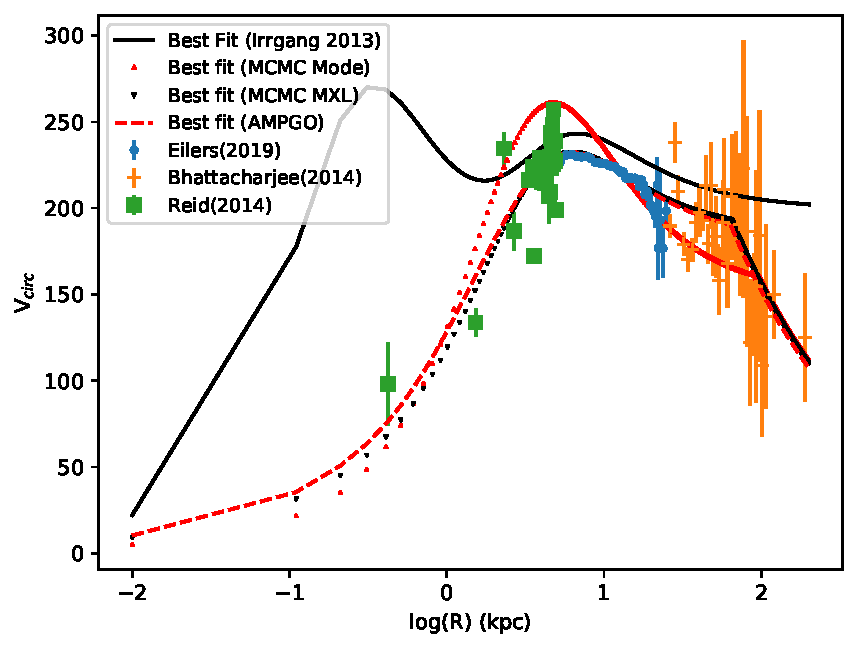
\includegraphics[width=\columnwidth]{Model_I/Plots/Reid(2014)/Rotcur_ModelI_eil_bhatta_log_10000_100.pdf}
\caption{The Rotation curve of the Milky Way in the Log scale for the best fit models and the original model 1 of Andreas for RC1 (top), RC2 (middle), and RC3 (bottom).
}
\label{fig:Model1_rc}
\end{figure}

\begin{figure}
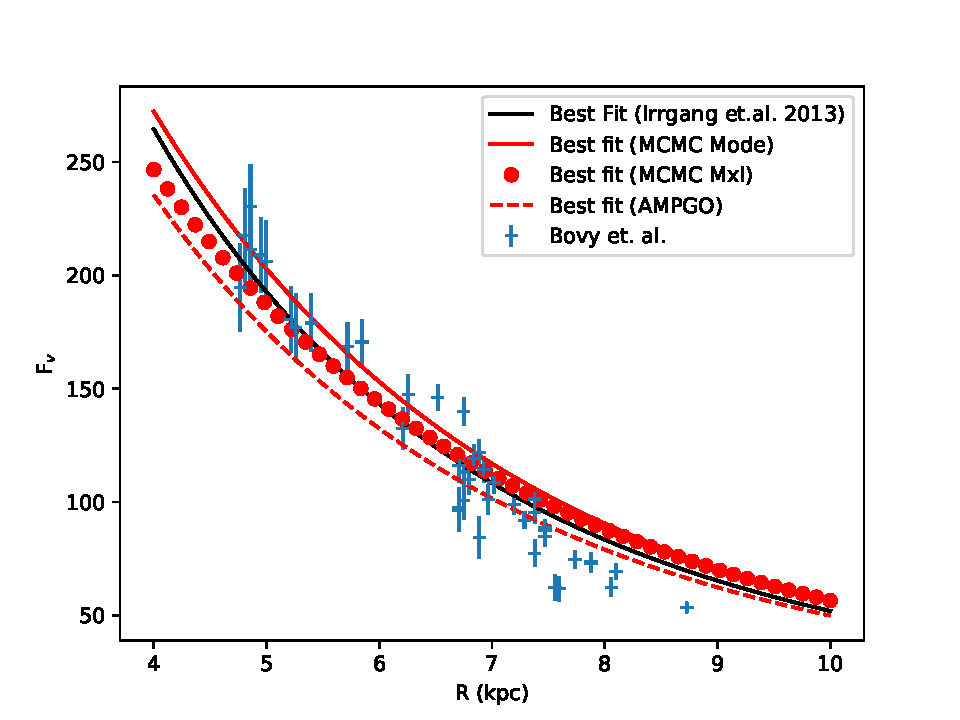
\includegraphics[width=\columnwidth]{Model_I/Plots/Sofue(2009)/VertForce_ModelI_10000_100.pdf}
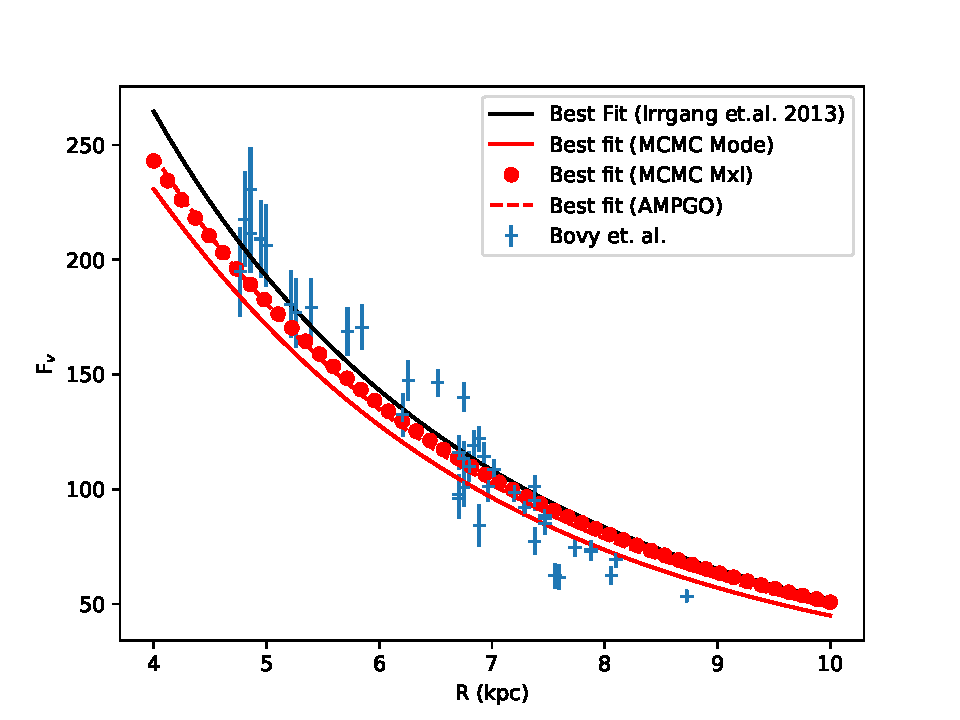
\includegraphics[width=\columnwidth]{Model_I/Plots/Sofue(2021)/VertForce_ModelI_10000_100.pdf}
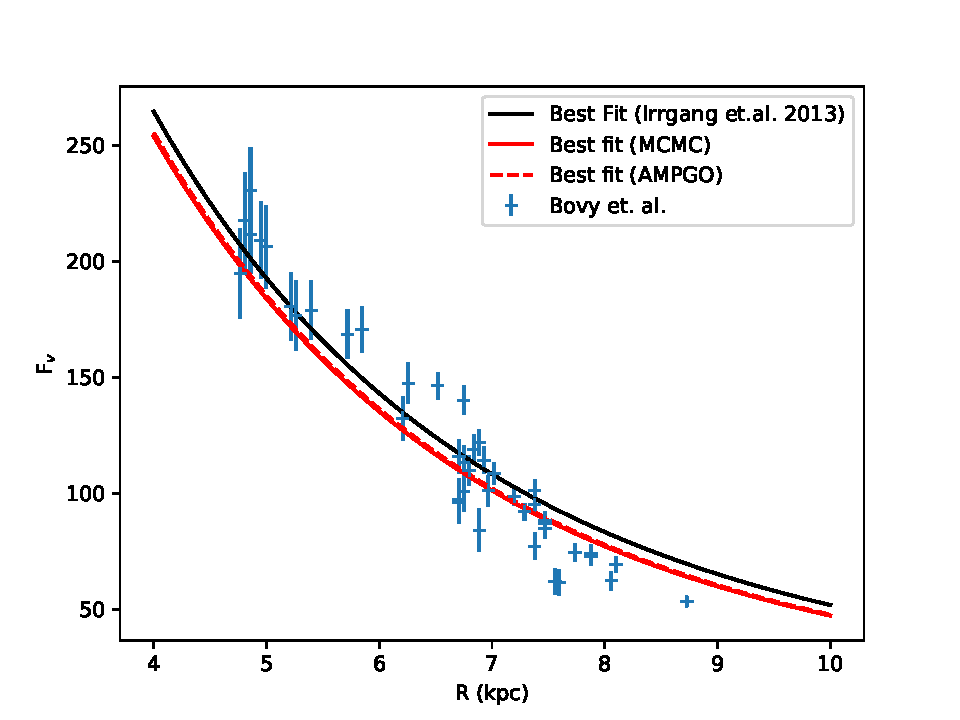
\includegraphics[width=\columnwidth]{Model_I/Plots/Reid(2014)/VertForce_ModelI_10000_100.pdf}
\caption{The Vertical force at 1.1 kpc for the best fit models and the original model 1 of Andreas.
}
\label{fig:Model1_vertif}
\end{figure}


\subsection{Model III: NFW Halo}

Model III of \citet{andreassmass} had the same bulge and disk components as Model I, but the Halo profile was that of \citet{1997ApJ...490..493N}. Due to the missing rotation curve outside the 25 kpc region, the values of Halo mass and scale were not properly constrained and Model I was favoured over Model III. However, as our rotation curve values include values outside of this region we are able to constrain this Halo profile in a much better manner. 

Like with Model I, Model III also has a bigger bulge preferred for RC2 and RC3. On the other hand the disk length and mass is fairly consistent, but the scale height is once again bigger than predicted before. For the halo, a denser region is preferred for all three curves, but especially for RC2 and RC3 where the constrained mass is much lower but the scale length is much bigger, and close to the maximum allowed value of 200 kpc (which is relevant for the upper bound errors). However the constrained mass still has big upper bounds, which is possibly due to the fact that outer halo rotation curve values are not as well constrained as the inside 25 kpc. 

The curves and fits are shown in \ref{fig:Model3_rc} and \ref{fig:Model3_vertif}.


\begin{figure}
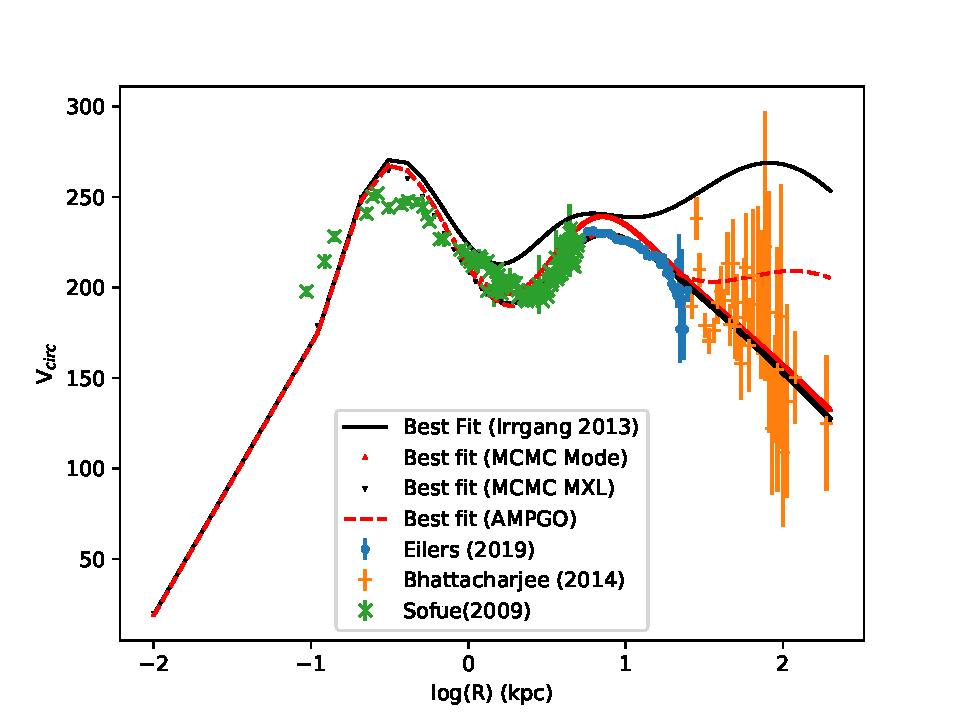
\includegraphics[width=\columnwidth]{Model_III/Plots/Sofue(2009)/Rotcur_ModelIII_log_10000_100.pdf}
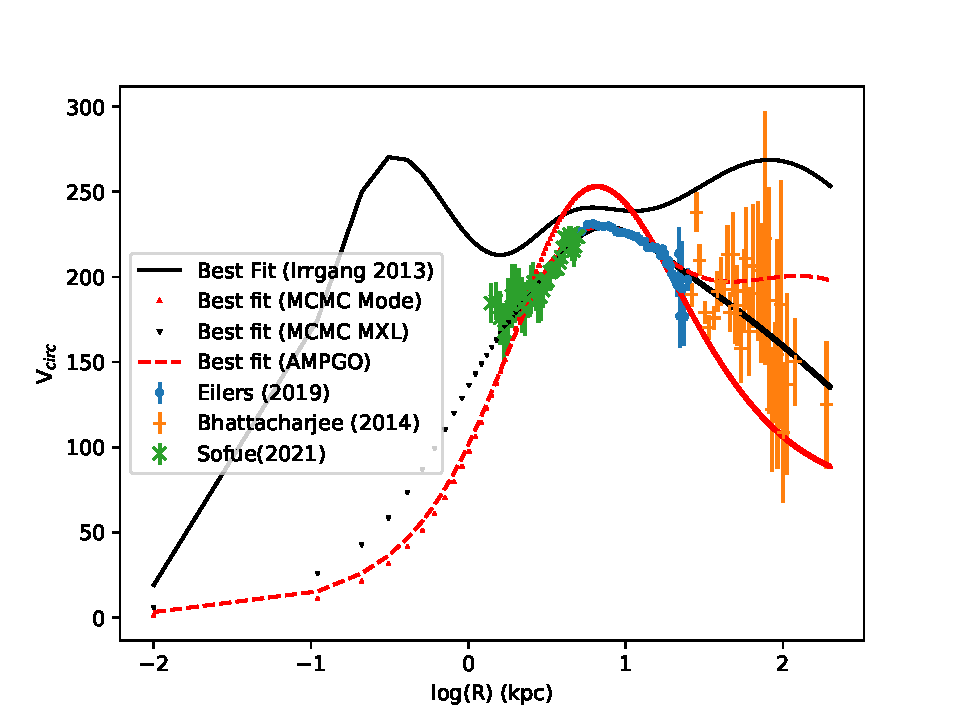
\includegraphics[width=\columnwidth]{Model_III/Plots/Sofue(2021)/Rotcur_ModelIII_log_10000_100.pdf}
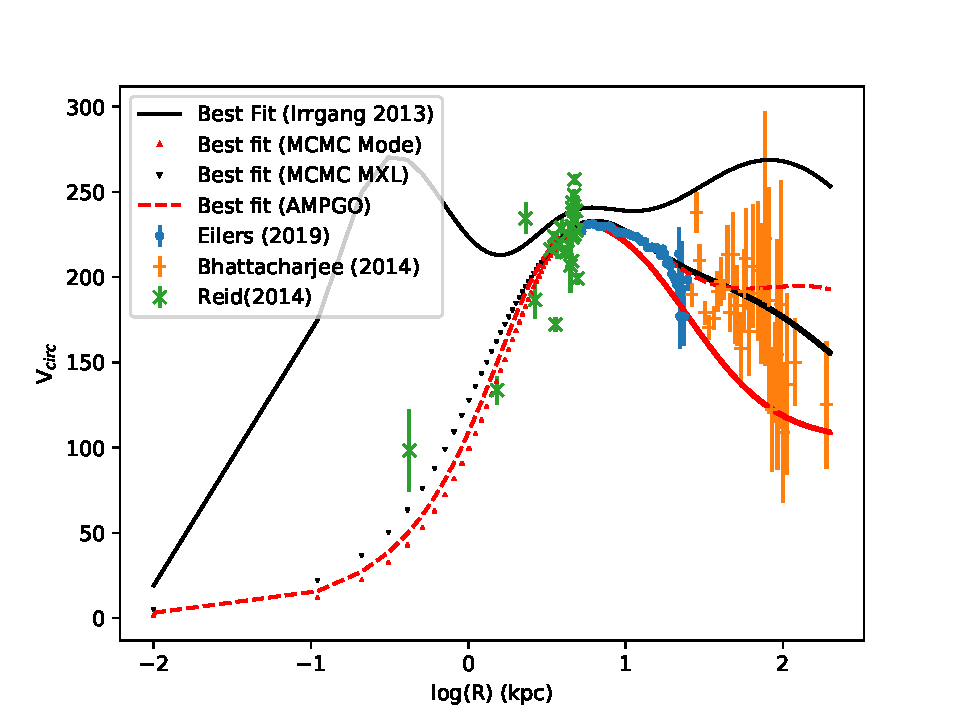
\includegraphics[width=\columnwidth]{Model_III/Plots/Reid(2014)/Rotcur_ModelIII_log_10000_100.pdf}
\caption{The Rotation curve of the Milky Way in the Log scale for the best fit models and the original model 1 of Andreas for RC1 (top), RC2 (middle), and RC3 (bottom).
}
\label{fig:Model3_rc}
\end{figure}
\begin{figure}
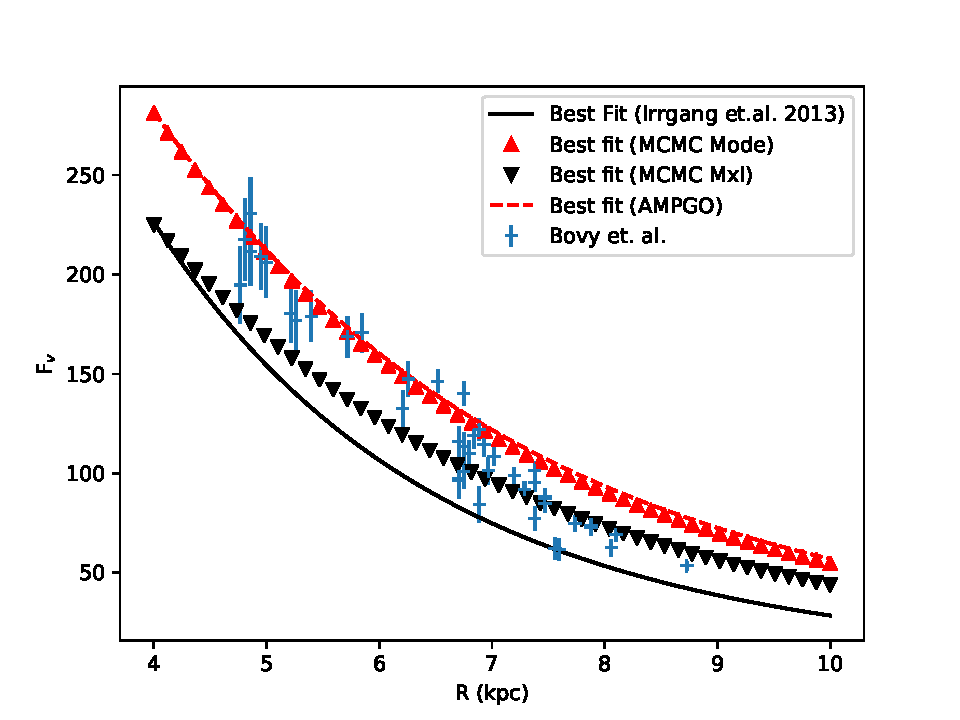
\includegraphics[width=\columnwidth]{Model_III/Plots/Sofue(2009)/VertForce_ModelIII_10000_100.pdf}
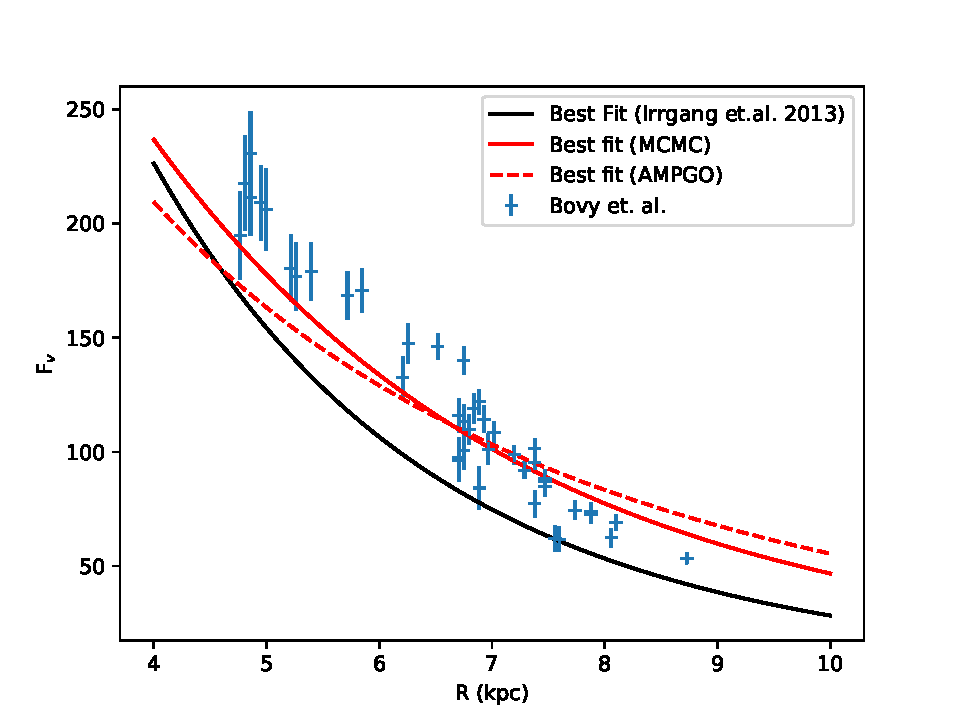
\includegraphics[width=\columnwidth]{Model_III/Plots/Sofue(2021)/VertForce_ModelIII_10000_100.pdf}
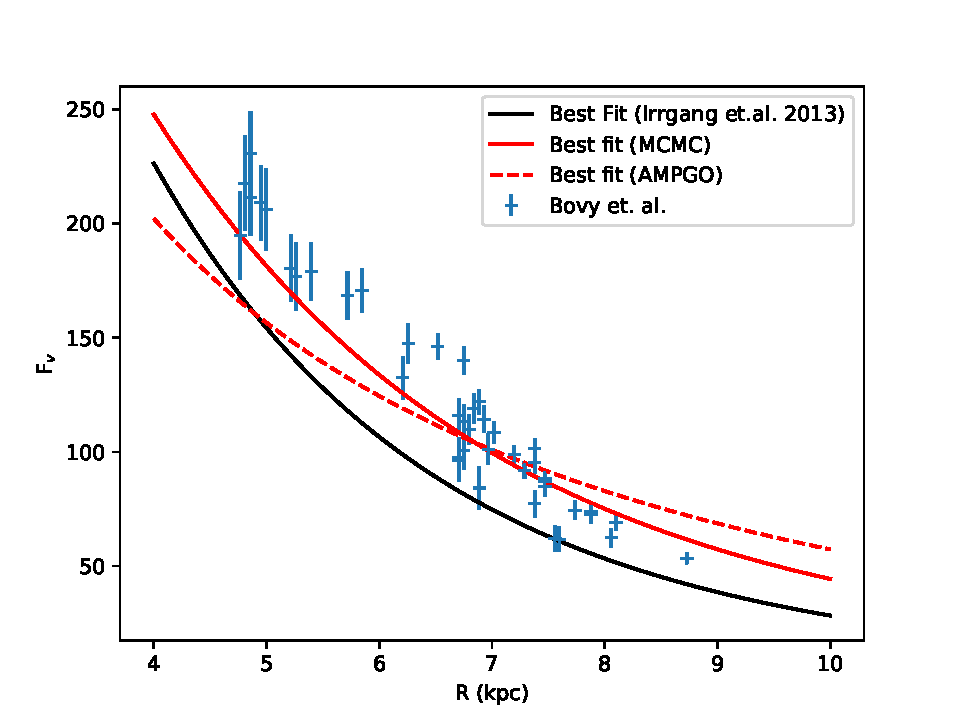
\includegraphics[width=\columnwidth]{Model_III/Plots/Reid(2014)/VertForce_ModelIII_10000_100.pdf}
\caption{The Vertical force at 1.1 kpc for the best fit models and the original model 1 of Andreas.
}
\label{fig:Model3_vertif}
\end{figure}
\begin{table*}
\begin{center}
\caption{Fitted parameters values for Model III. Values given are the Mode and HDI of the posterior parameter distributions. }\label{tab:model3params} 
%\scriptsize
\renewcommand{\arraystretch}{1.3}
\begin{tabular}{c c c c c } 
\hline
\hline
&\multicolumn{4}{c}{Model III} \\
\hline
Parameter&Old&RC1&RC2&RC3\\
\hline
$M_b$&$439^{+28}_{-28}$&$451^{+73}_{-65} (458^{+74}_{-64})$&$4335^{+797}_{-2423} (3237^{1425}_{-1950})$&$4326^{+662}_{-1896} (3568^{+1063}_{-1694})$\\
$b_b$&$0.236^{0.021}_{-0.021}$&$0.247^{+0.043}_{-0.043} (0.249^{0.045}_{-0.040})$&$3.480^{+0.853}_{-0.967} (3.303^{+0.759}_{-1.206})$&$3.427^{+0.556}_{-0.856} (3.209^{+0.579}_{-0.925})$\\
$M_d$&$3096^{+197}_{-197}$&$5593^{+757}_{-680} (5647^{+735}_{-702})$&$5332^{+1997}_{-1762} (5785^{+2324}_{-1662})$&$5002^{+2758}_{-1633} (5947^{+2964}_{-1856})$\\
$a_d$&$3.262^{+0.144}_{-0.121}$&$3.957^{+0.370}_{-0.410} (3.942^{+0.389}_{-0.390})$&$4.345^{+7.913}_{-1.149} (8.704^{+6.947}_{-4.050})$&$6.245^{+7.756}_{-3.068} (10.489^{+6.209}_{-5.119})$\\
$b_d$&$0.289^{+0.022}_{-0.022}$&$1.332^{+0.501}_{-0.376} (1.402^{+0.455}_{-0.423})$&$1.230^{+0.477}_{-0.935} (1.120^{+0.722}_{-0.702})$&$1.008^{+0.583}_{-0.793} (1.052^{+0.749}_{-0.666})$\\
$M_h$&$142200^{+137900}_{-75500}$&$141781^{+353748}_{-87253} (335899^{+266194}_{-207039})$&$23070^{+260397}_{-23065} (181037^{+243432}_{-131116})$&$20600^{+247585}_{-20599} (167527^{+242697}_{-124304})$\\
$a_h$&$45.02^{22.56}_{-16.78}$&$192.232^{+7.758}_{-74.180} (146.574^{+39.161}_{-61.570})$&$193.341^{+6.659}_{-63.225} (154.766^{+32.821}_{-55.782})$&$192.977^{+7.022}_{-66.802} (152.021^{+35.181}_{-58.017})$\\
\hline
$\chi^2_{\text{Reduced}}$&&0.05&0.044&0.06  \\
\end{tabular}
\end{center}
\end{table*}

\section{Comparisons and analysis of predicted quantities}

A big takeaway though is that for all three curves (along with the vertical force), Model III has much better reduced $\chi^2$ values, and is therefore preferred over Model I.




\bibliographystyle{mnras}
\bibliography{references.bib} % if your bibtex file is called example.bib


\appendix
\section{Math}

The bulge is given by:

\section{Correlations - ModelI}

\begin{figure}
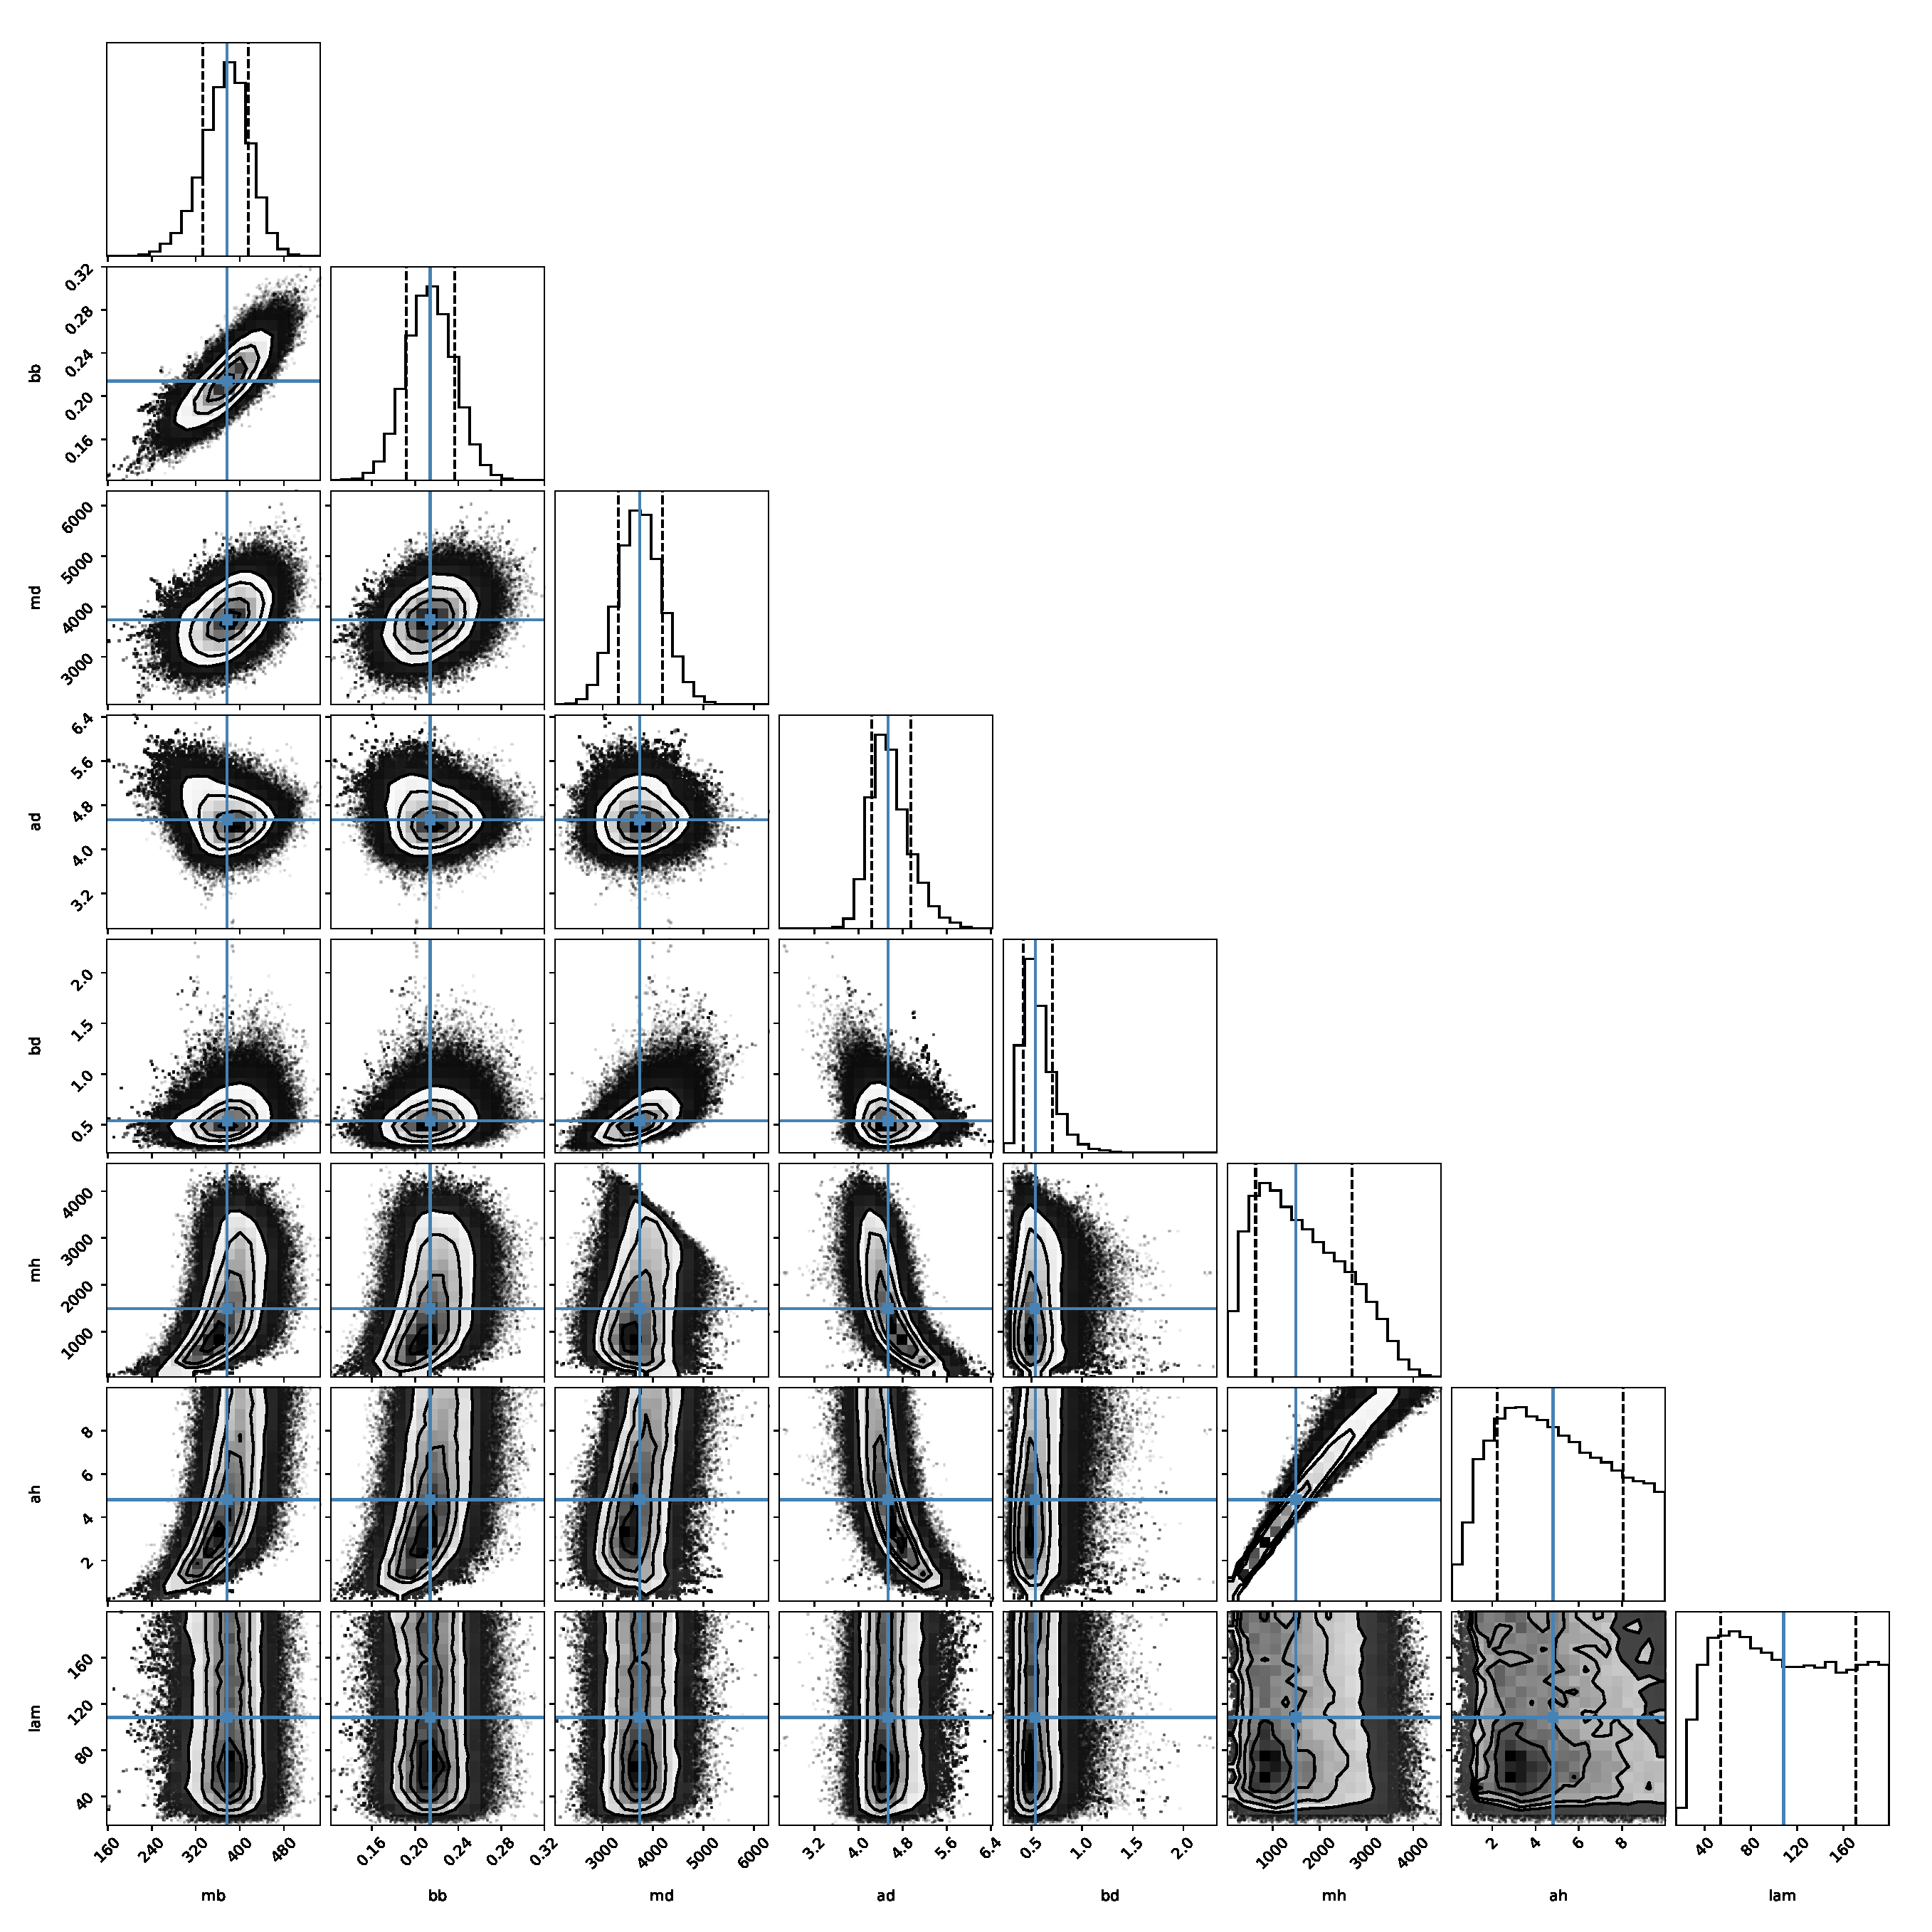
\includegraphics[width=\columnwidth]{Model_I/Plots/Sofue(2009)/emcee_corner_10000_100.pdf}
\caption{Correlations for RC1
}
\label{fig:Model1_Sofue2009}
\end{figure}

\begin{figure}
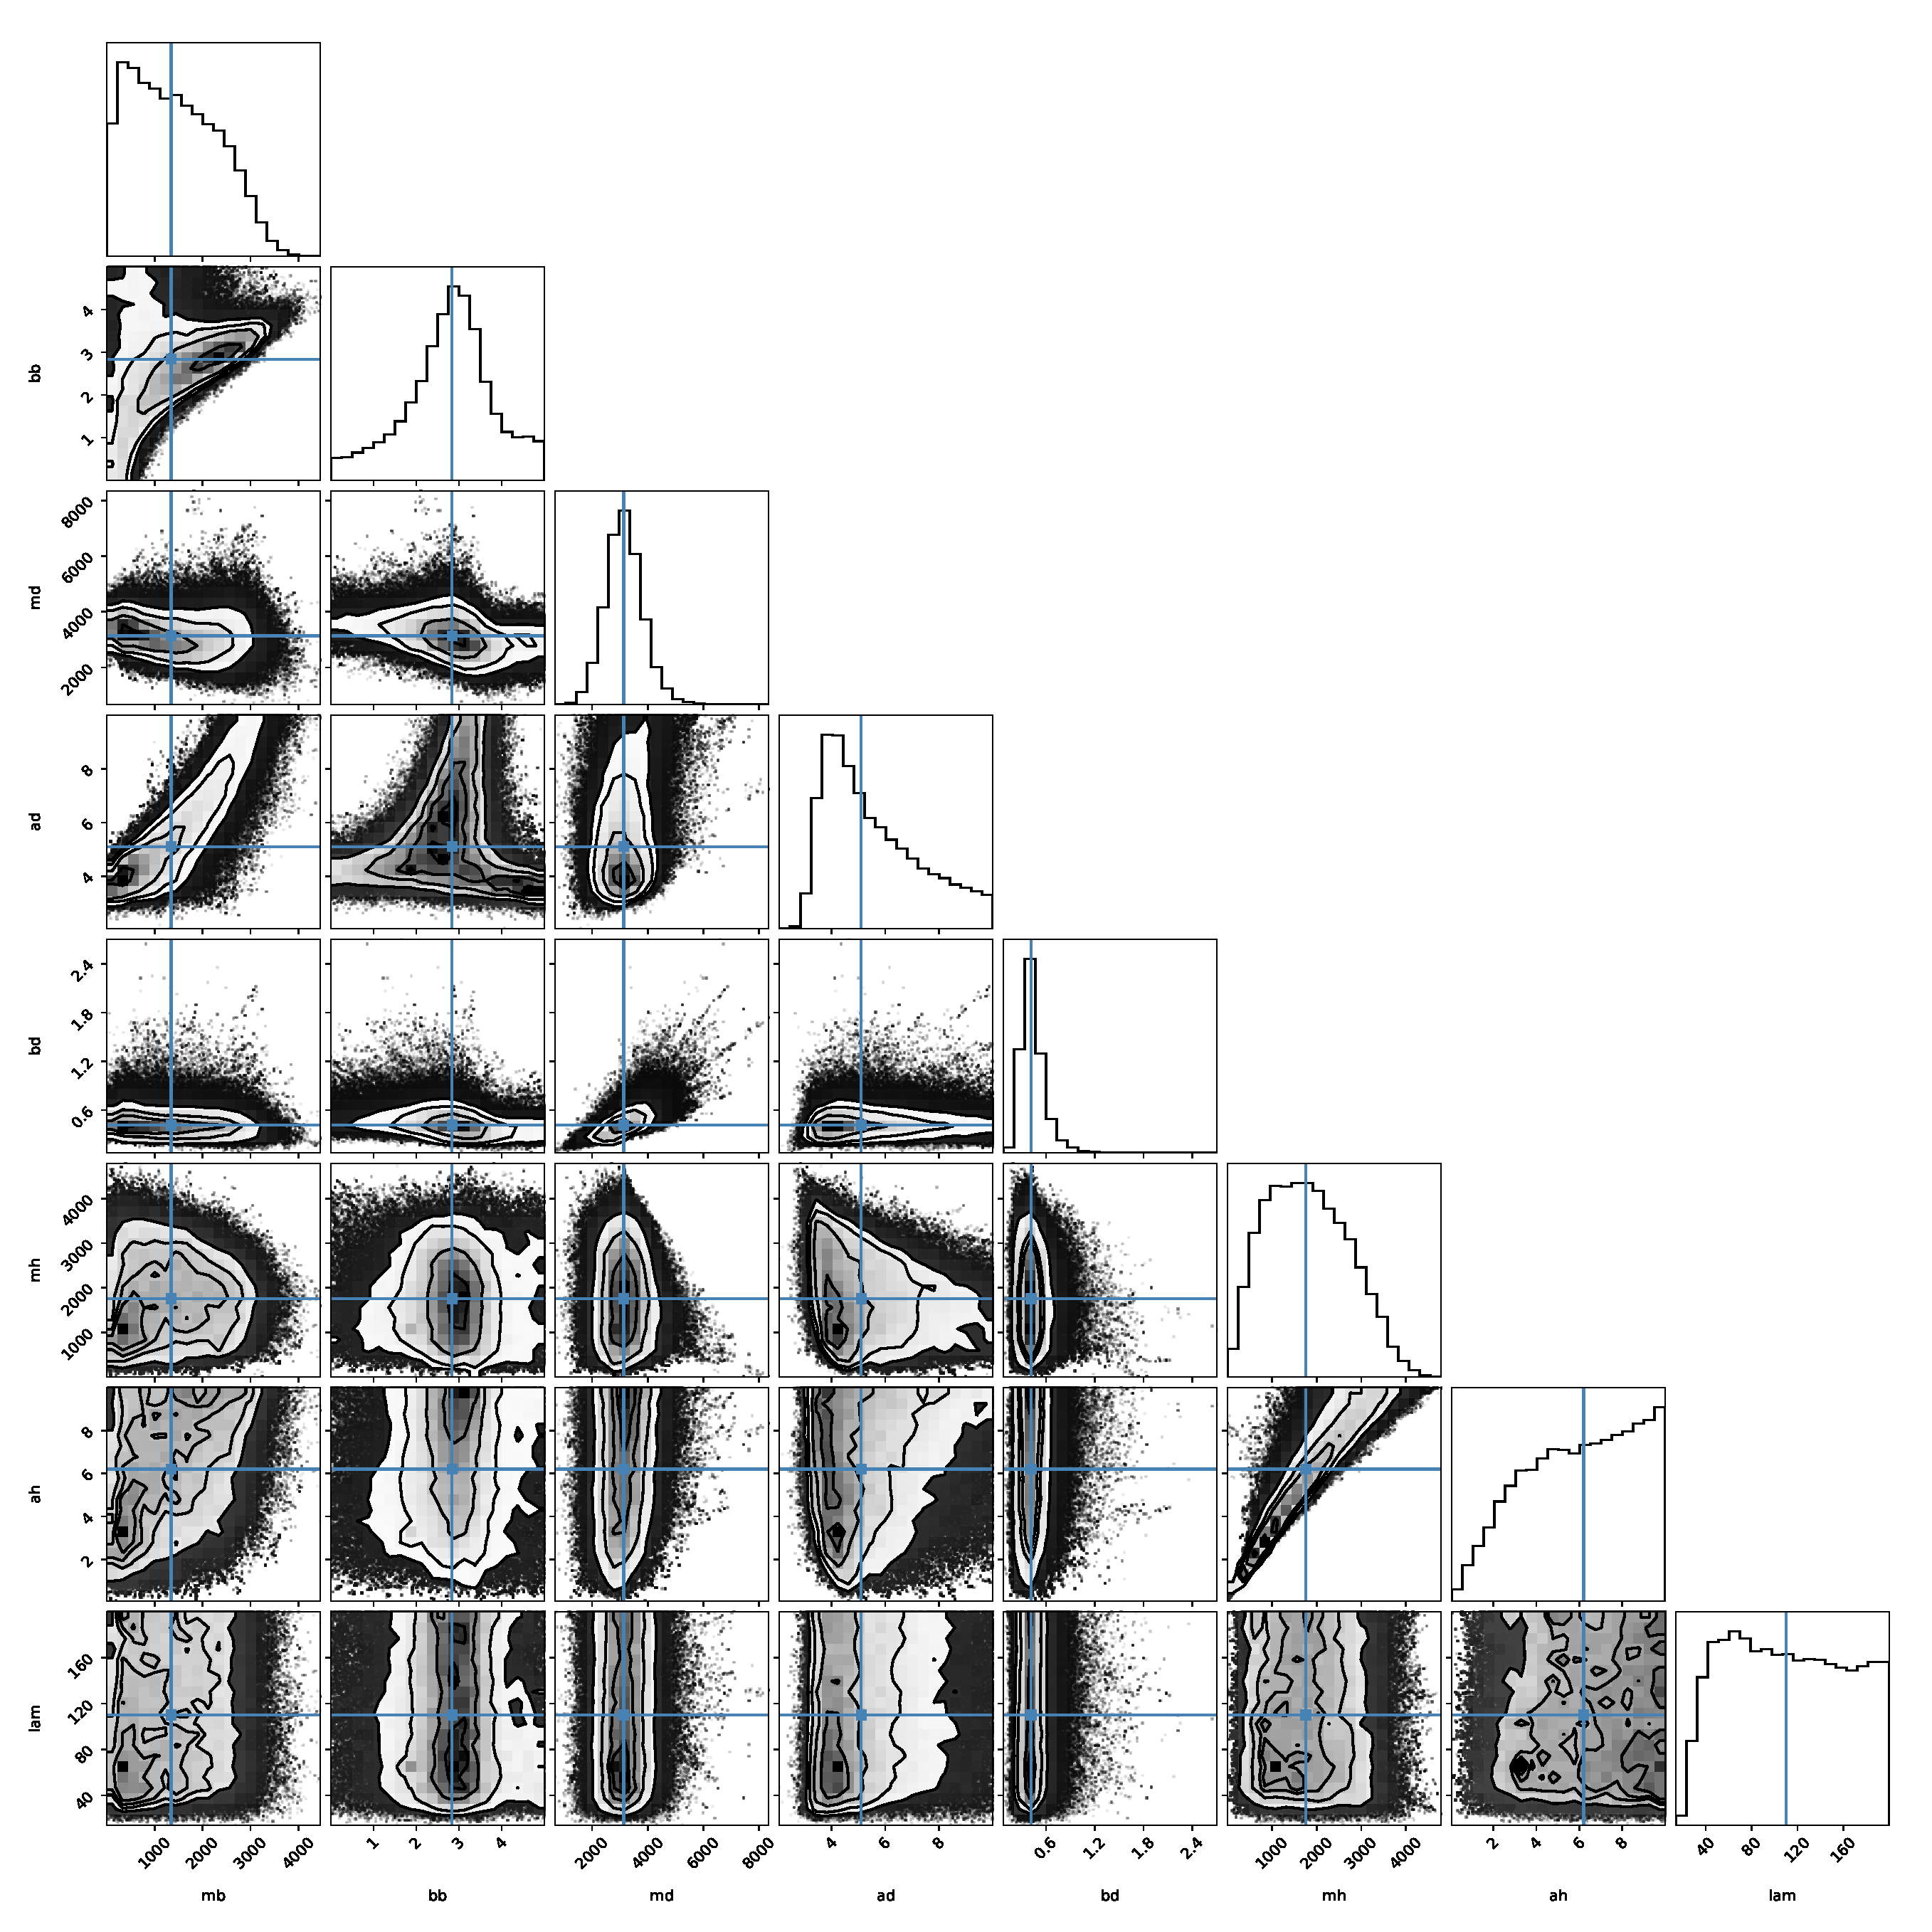
\includegraphics[width=\columnwidth]{Model_I/Plots/Sofue(2021)/emcee_corner_10000_100.pdf}
\caption{Correlations for Sofue 2021
}
\label{fig:Model1_Sofue2021}
\end{figure}

\begin{figure}
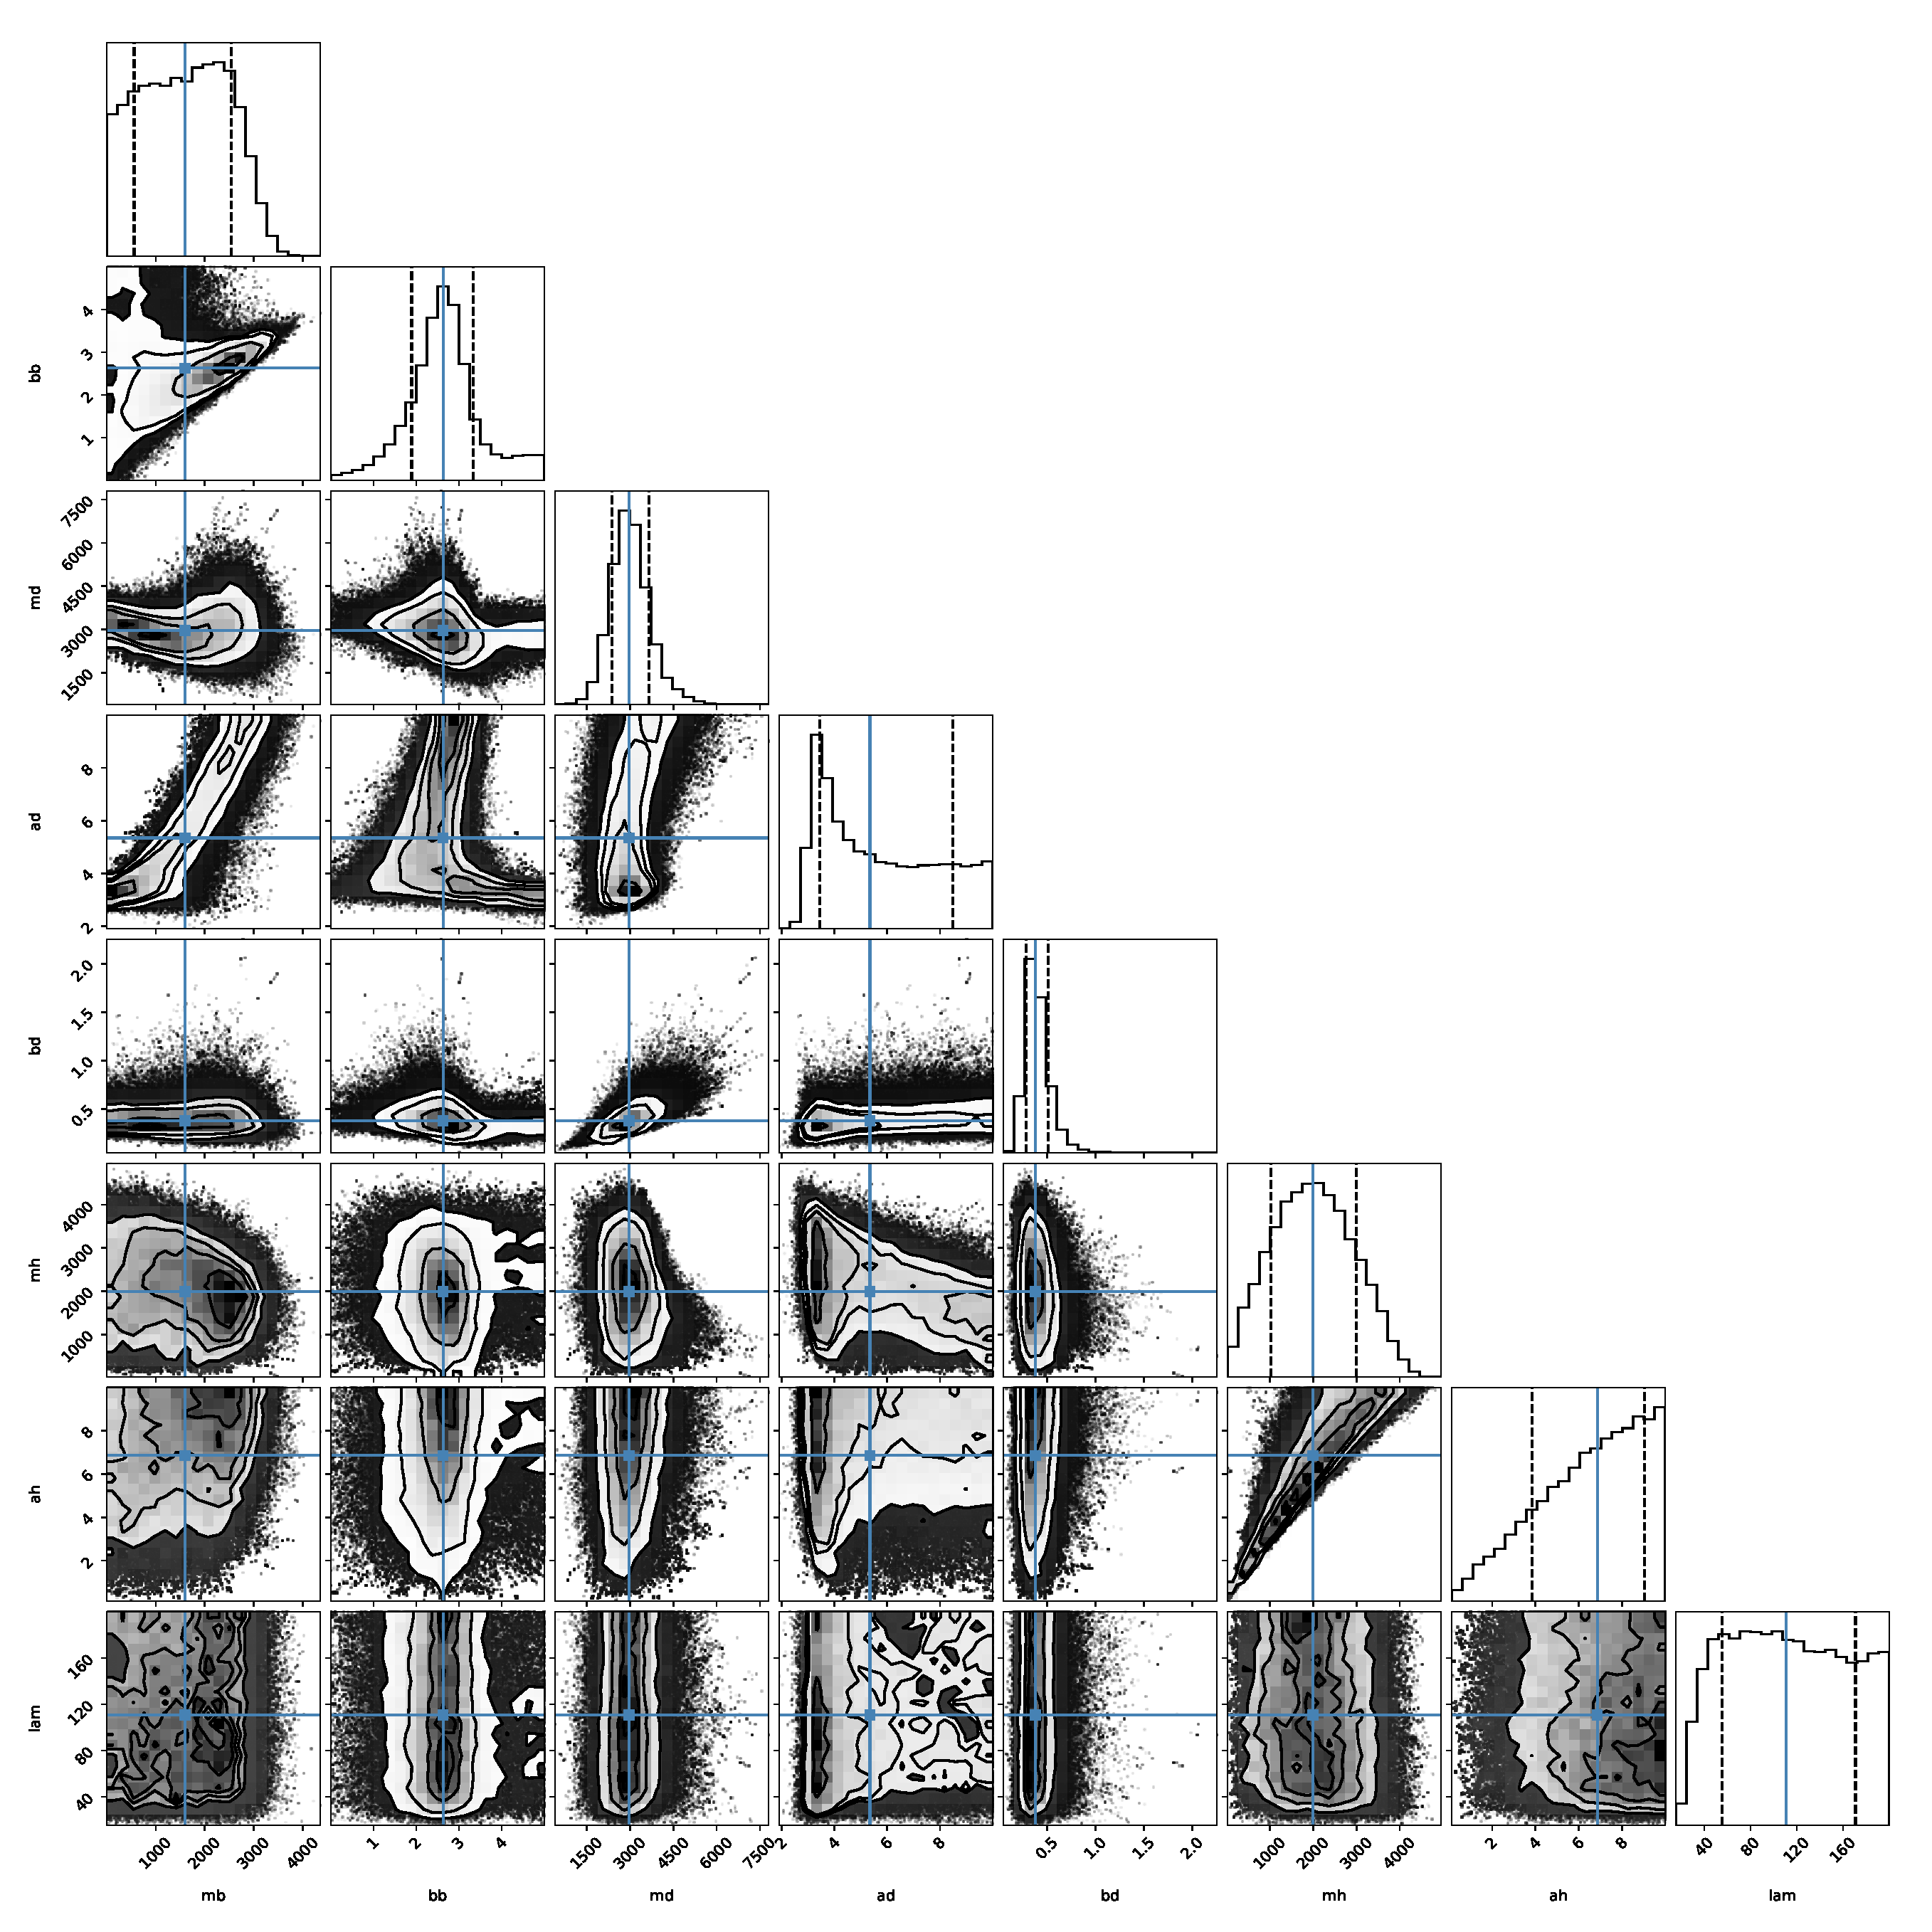
\includegraphics[width=\columnwidth]{Model_I/Plots/Reid(2014)/emcee_corner_10000_100.pdf}
\caption{Correlations for Reid 2014
}
\label{fig:Model1_Reid2014}
\end{figure}
\section{Correlations - ModelIII}

\begin{figure}
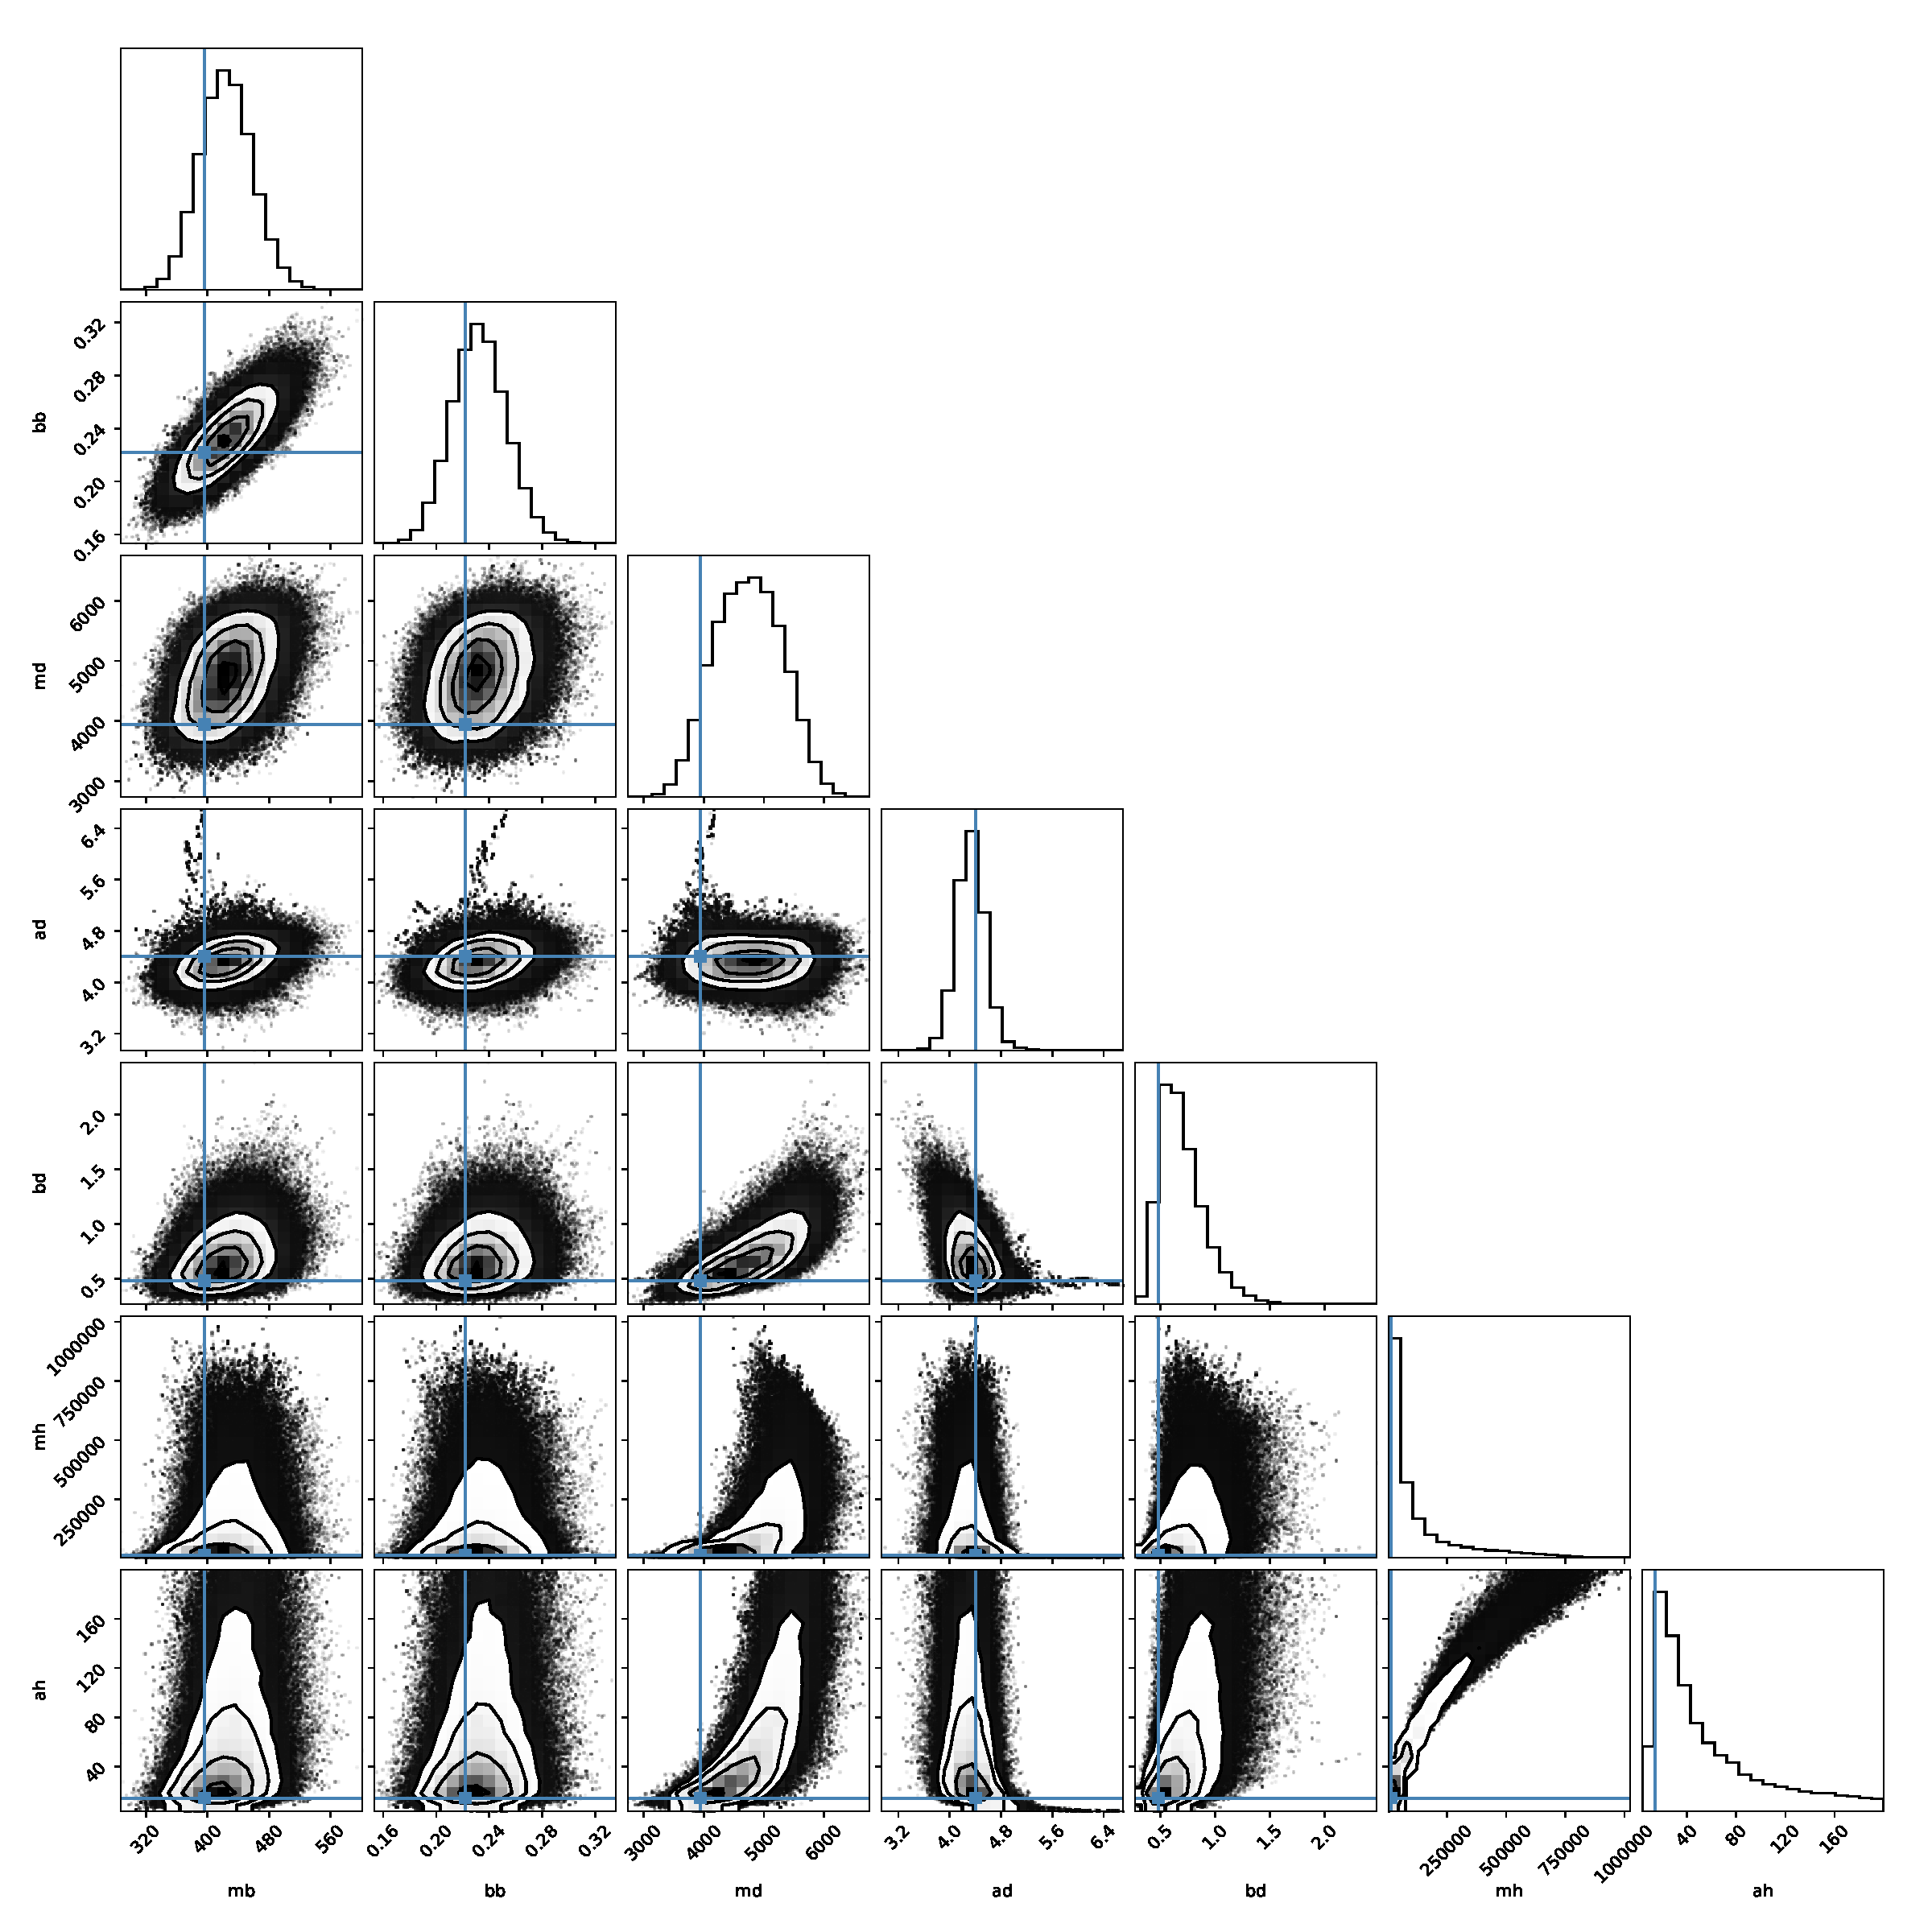
\includegraphics[width=\columnwidth]{Model_III/Plots/Sofue(2009)/emcee_corner_10000_100.pdf}
\caption{Correlations for RC1
}
\label{fig:Model3_Sofue2009}
\end{figure}

\begin{figure}
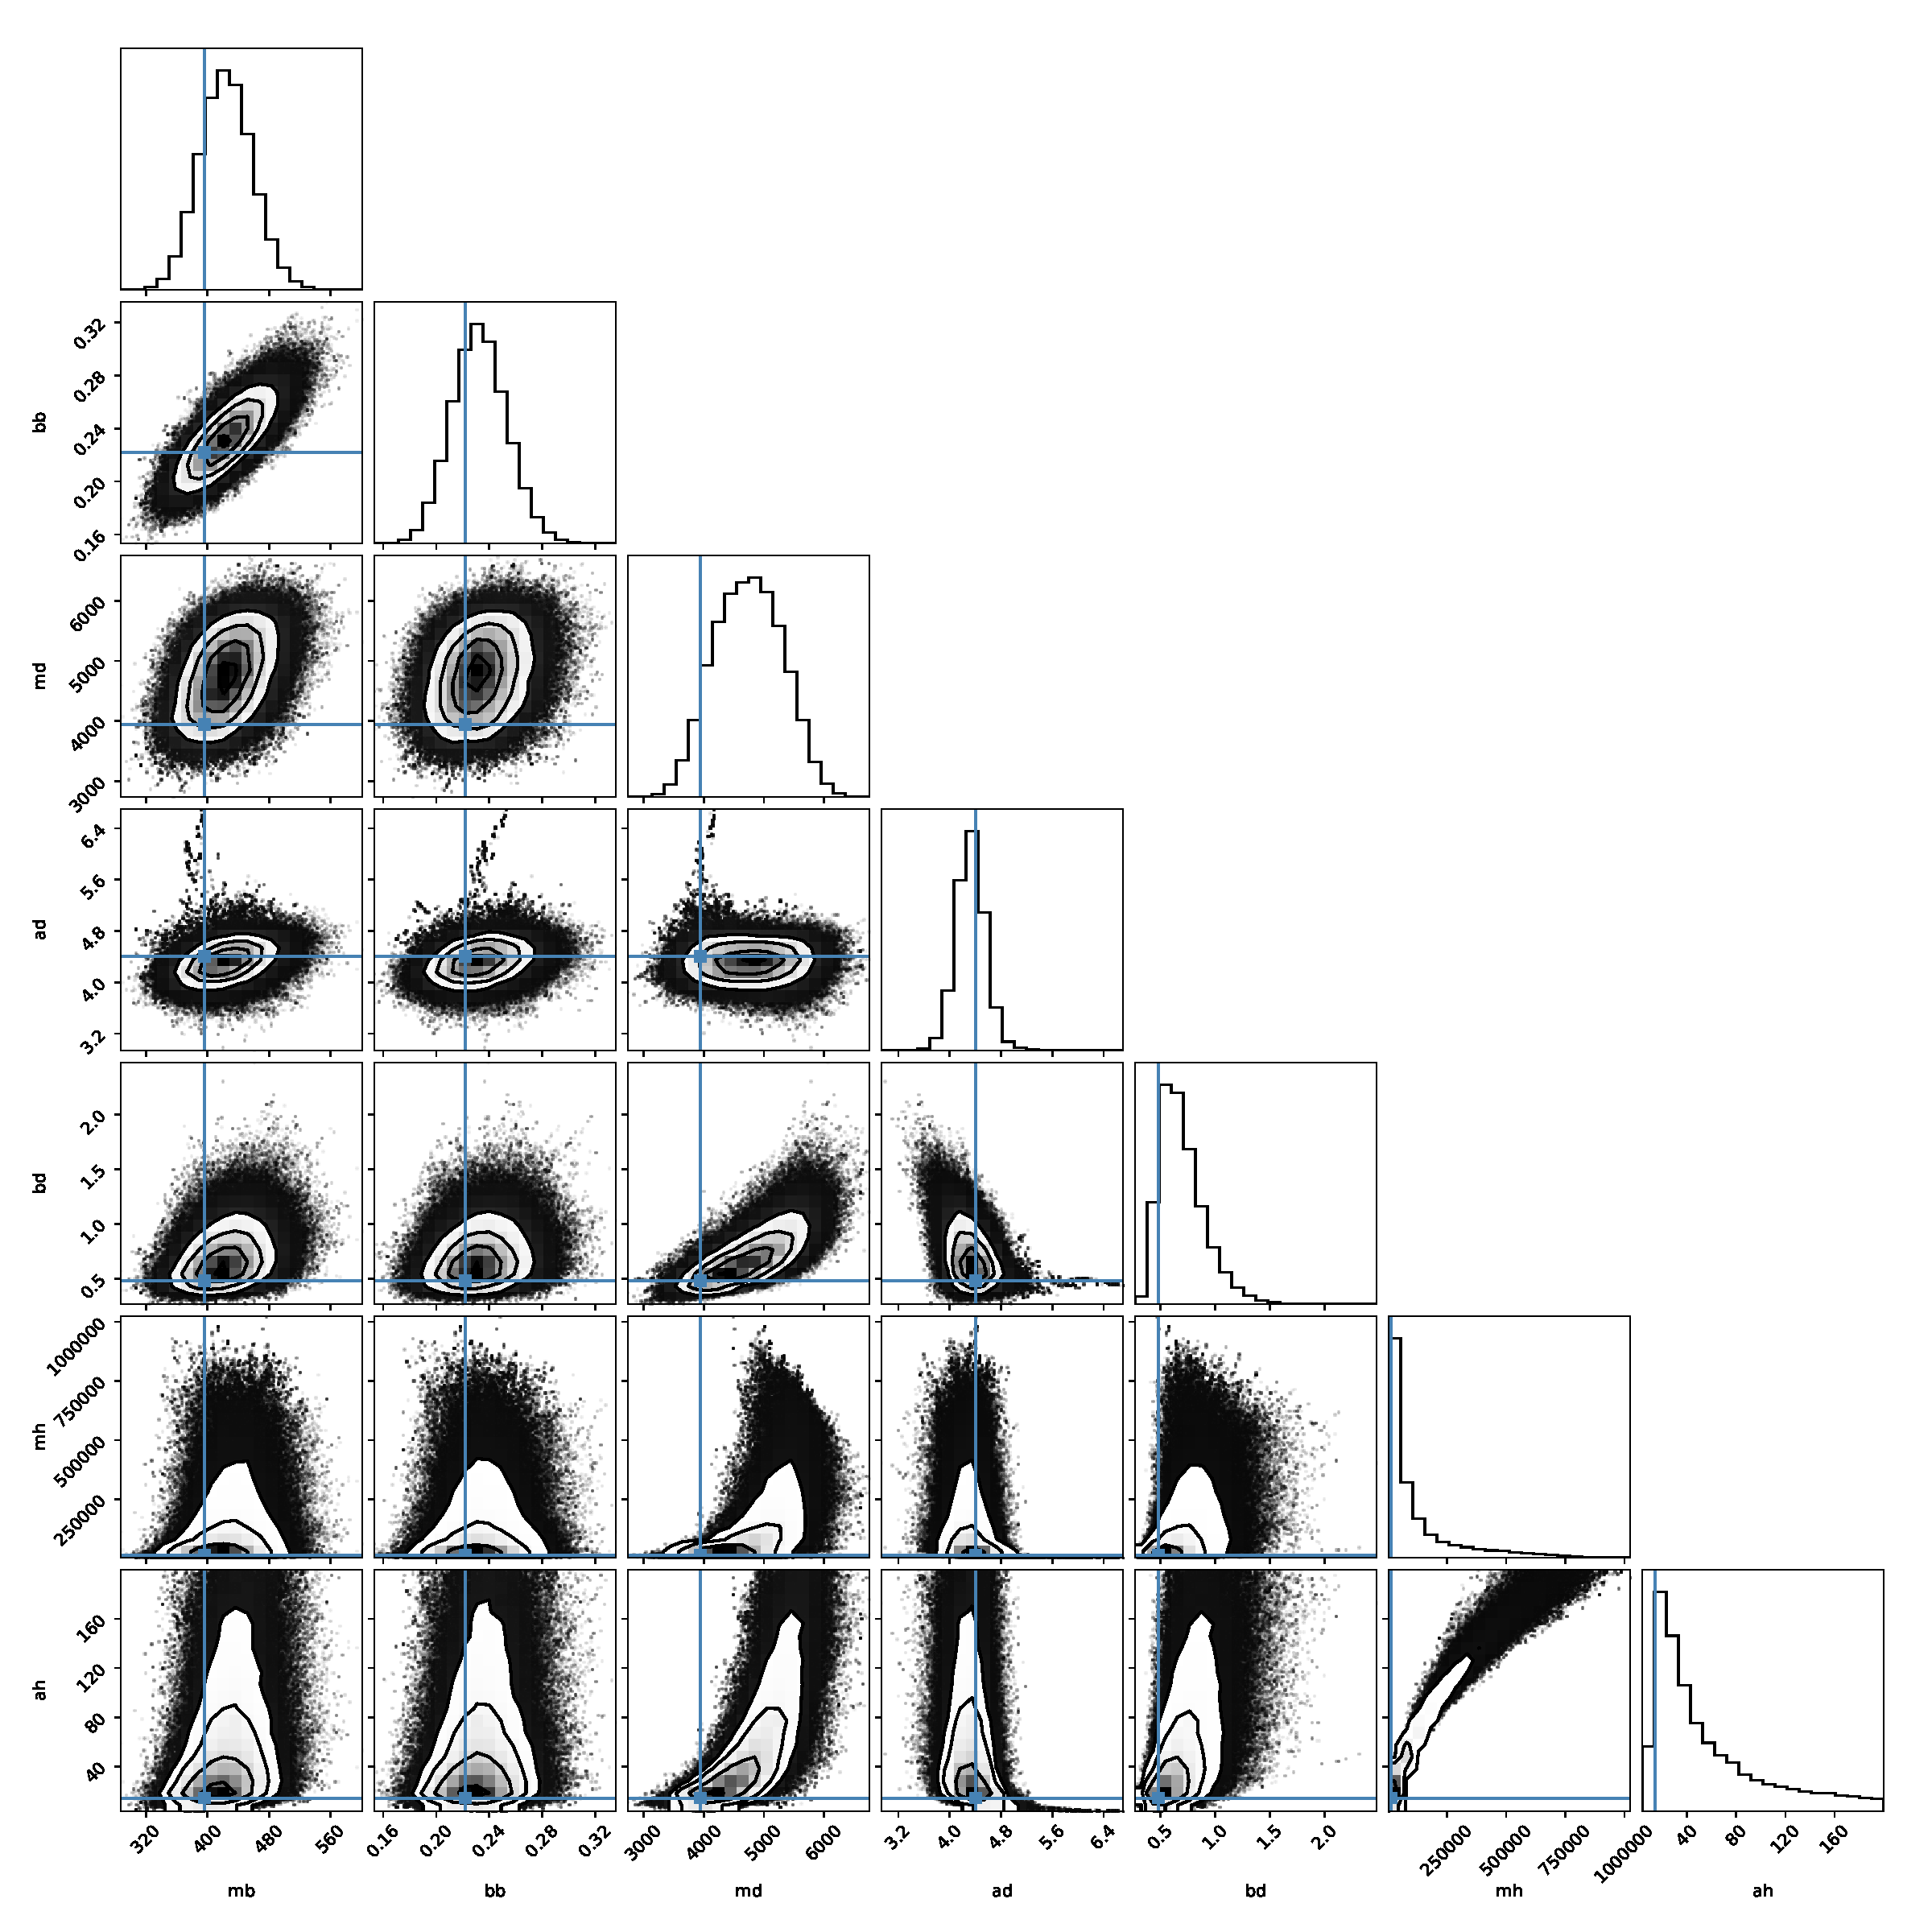
\includegraphics[width=\columnwidth]{Model_III/Plots/Sofue(2009)/emcee_corner_10000_100.pdf}
\caption{Correlations for Sofue 2021
}
\label{fig:Model3_Sofue2021}
\end{figure}

\begin{figure}
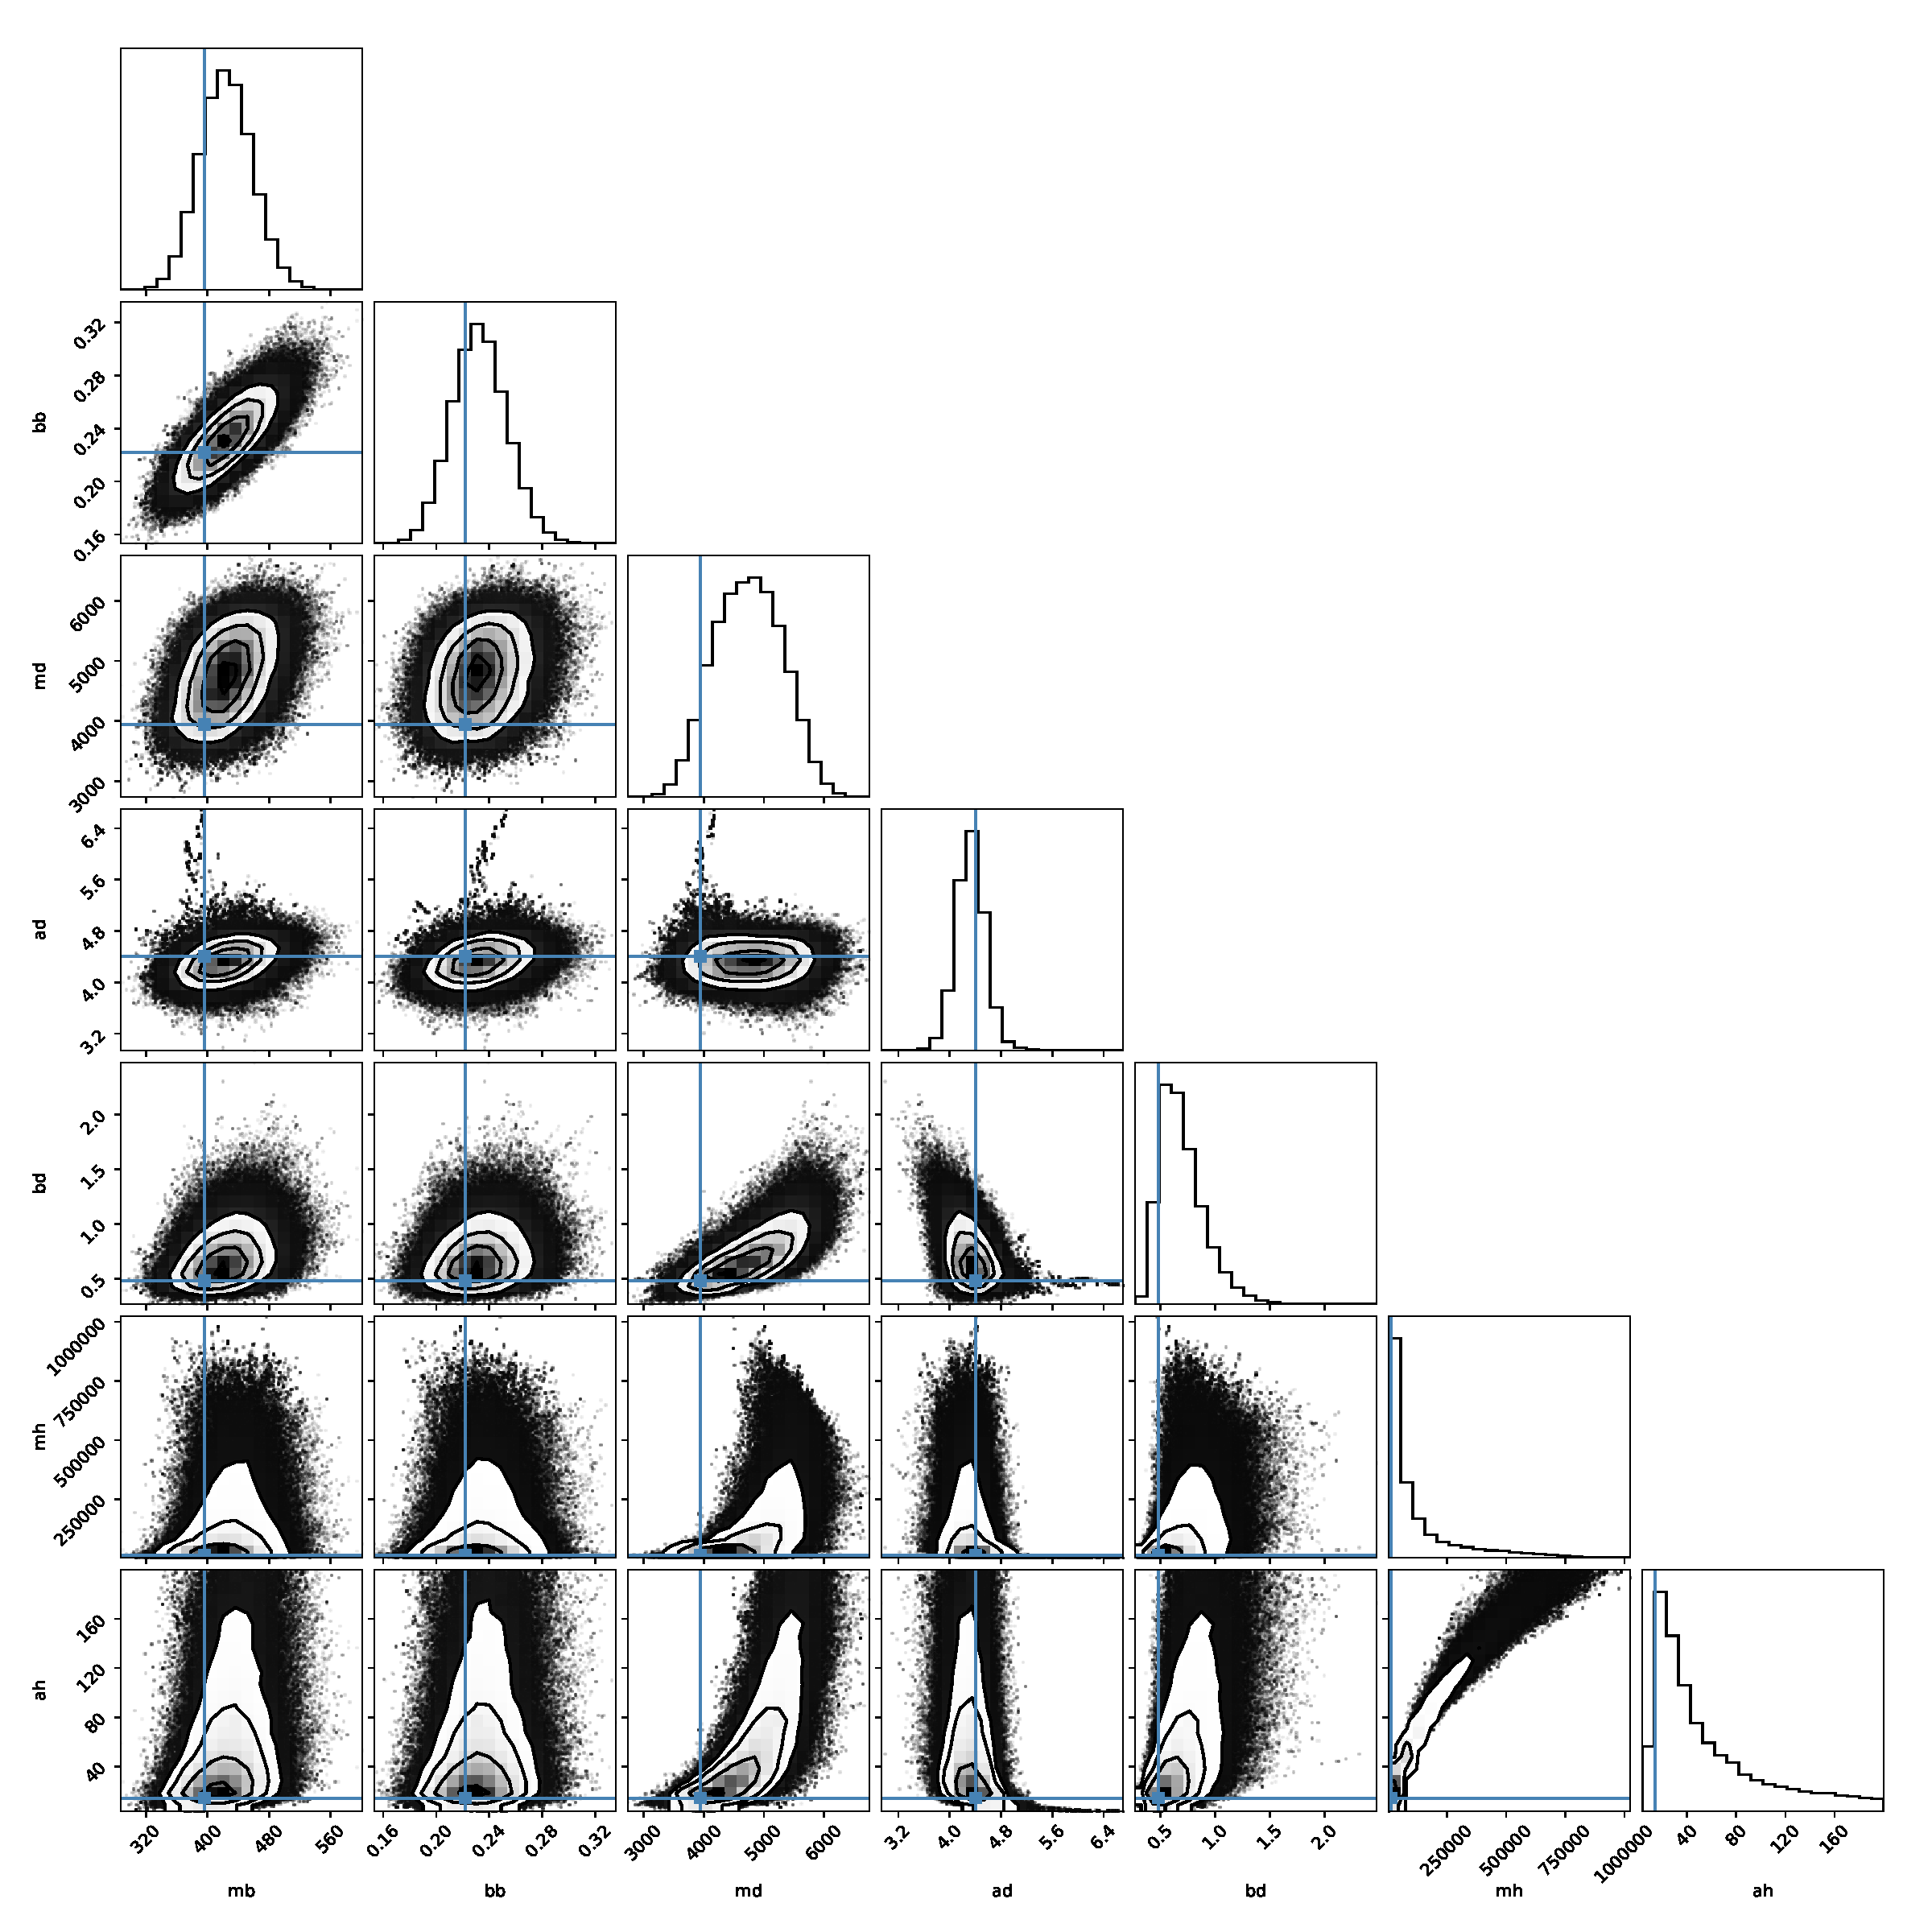
\includegraphics[width=\columnwidth]{Model_III/Plots/Sofue(2009)/emcee_corner_10000_100.pdf}
\caption{Correlations for Reid 2014
}
\label{fig:Model3_Reid2014}
\end{figure}
\bsp	% typesetting comment
\label{lastpage}
\end{document}